\documentclass[18pt]{beamer}
\usepackage{tcolorbox}
\usepackage{templates/beamerthemekitwide}
\usepackage{ifthen}
\usepackage{pdfpages}
\usepackage{pifont}
\usepackage{hyperref}
\usepackage[autostyle]{csquotes}
\usepackage[hyperref,backend=biber,url=false]{biblatex}
\usepackage{pgfplots}
\pgfplotsset{compat=1.16}
\usepgfplotslibrary{statistics}
\usepackage{tikz}
\usetikzlibrary{decorations.pathreplacing,shapes,positioning}
\usepackage{siunitx}
\usepackage{marvosym}
\usepackage[clock]{ifsym}

\title[Analysis and Optimization of AVX DVFS]{Analysis and Optimization of Dynamic Voltage and Frequency Scaling for AVX Workloads Using a Software-Based Reimplementation}
\author{Yussuf Khalil}
\date{25 September 2019}
\institute{Operating Systems Group}

\addbibresource{presentation.bib}

\selectlanguage{english}

\definecolor{kitgreenexcl}{cmyk}{1.0,  0.0,  0.6, 0.0}
\definecolor{kitblue}     {cmyk}{0.8,  0.5,  0.0, 0.0}
\definecolor{kitgreen}    {cmyk}{0.6,  0.0,  1.0, 0.0}
\definecolor{kityellow}   {cmyk}{0.0,  0.05, 1.0, 0.0}
\definecolor{kitorange}   {cmyk}{0.0,  0.45, 1.0, 0.0}
\definecolor{kitbrown}    {cmyk}{0.35, 0.5,  1.0, 0.0}
\definecolor{kitred}      {cmyk}{0.25, 1.0,  1.0, 0.0}
\definecolor{kitpurple}   {cmyk}{0.25, 1.0,  0.0, 0.0}
\definecolor{kitcyan}     {cmyk}{0.9,  0.05, 0.0, 0.0}
\definecolor{kitgrey}	  {cmyk}{0.0,  0.0,  0.0, 0.15}
\definecolor{kitdarkgrey} {cmyk}{0.0,  0.0,  0.0, 0.5}

% https://tex.stackexchange.com/a/47797
\tikzset{ref/.style={insert path={%
			coordinate [pos=0,xshift=-0.5\pgflinewidth,yshift=-0.5\pgflinewidth] (#1 south west)
			coordinate [pos=1,xshift=0.5\pgflinewidth,yshift=0.5\pgflinewidth]   (#1 north east)
			coordinate [pos=.5] (#1 center)
			(#1 south west |- #1 north east)     coordinate (#1 north west)
			(#1 center     |- #1 north east)     coordinate (#1 north)
			(#1 center     |- #1 south west)     coordinate (#1 south)
			(#1 south west -| #1 north east)     coordinate (#1 south east)
			(#1 center     -| #1 south west)     coordinate (#1 west)
			(#1 center     -| #1 north east)     coordinate (#1 east)
}}}

\begin{document}
\selectlanguage{english}

\begin{frame}
	\titlepage
\end{frame}

\section{Motivation}
\begin{frame}[t]{Motivation}
	\begin{itemize}
		\item AVX is a modern vector processing extension for x86 processors
		\item Current Intel CPUs reduce their clock frequency when executing AVX code
		\item Lowered frequencies attained for a while after last AVX instruction
		\begin{itemize}
			\item[$\Rightarrow$] negative impact on performance in heterogeneous workloads
		\end{itemize}
	\end{itemize}
	\pause
	\begin{figure}
		\centering
		\vspace*{-0.7em}
		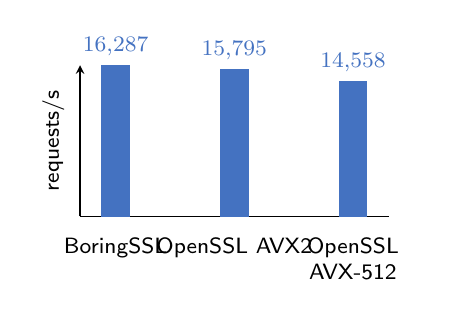
\begin{tikzpicture}[font=\footnotesize]
			\sffamily
			\begin{axis}[
				symbolic x coords={BoringSSL, OpenSSL AVX2, OpenSSL AVX-512},
				xtick=data,
				x tick label style  = {text width=2cm, align=center},
				ylabel={requests/s},
				axis y line=left,
				axis x line*=bottom,
				height=3.5cm,
				width=5.5cm,
				nodes near coords,
				ymin=0,
				ybar,
				enlarge x limits={0.15},
				ytick=\empty,
				xtick style={draw=none},
			]
			\addplot[fill=kitblue, color=kitblue] coordinates {
				(BoringSSL, 16287)
				(OpenSSL AVX2, 15795)
				(OpenSSL AVX-512, 14558)
			};
			\end{axis}
		\end{tikzpicture}
		\vspace*{-0.7em}
		\caption{nginx throughput with different ChaCha20-Poly1305 implementations\footfullcite{cloudflareinteldangers}}
	\end{figure}
\end{frame}

\section{Idea}
\begin{frame}[t]{Idea}
	\begin{itemize}
		\item Frequency switches are costly
		\begin{itemize}
			\item[$\Rightarrow$] wait before raising frequency after AVX execution
		\end{itemize}
		\pause
		\item What if we could predict when AVX code will be executed again?
		\item Could we raise the frequency earlier and improve performance during scalar phases?
		\item Similar approaches are used for device power management
	\end{itemize}
	\pause
	\begin{center}
		\vspace{1em}
		Try different reclocking algorithms!
	\end{center}
\end{frame}

\begin{frame}[t]{Idea}
	\begin{itemize}
		\item AVX reclocking is controlled solely by CPU itself
		\begin{itemize}
			\item We can not modify the hardware
			\begin{itemize}
				\item But we can (mostly) disable automatic reclocking
			\end{itemize}
			\item[$\Rightarrow$] reimplement algorithm in software
		\end{itemize}
		\pause
		\item Intel only provides vague description of algorithm\footfullcite{inteloptimizationmanual}
		\begin{itemize}
			\item Downclocking after $\leq$ \SI{500}{\micro\second}
			\item Upclocking after \SI{2}{\milli\second}
			\item Two frequency levels (\enquote{turbo licenses})
			\item[$\Rightarrow$] need to analyze what processors really do
		\end{itemize}
	\end{itemize}
\end{frame}
\chapter{Analysis}
\label{sec:analysis}

In order to be able to evaluate potential means of improving Intel's \gls{AVX} reclocking algorithm, we first need to obtain thorough knowledge of the algorithm as it is implemented in current Intel x86 \glspl{CPU}. We can then use this knowledge for the software-based reimplementation presented in \Cref{sec:design} and to understand the hardware-induced constraints Intel needs to keep within, which is in turn necessary for designing a feasible and implementable improved reclocking algorithm.

Intel regularly publishes optimization manuals~\cite{inteloptimizationmanual} intended for compiler developers and software engineers which contain a vague description of the mechanism used for deciding when to lower or raise the processor's frequency upon execution of \gls{AVX} instructions. Precisely, Intel defines three \textit{turbo license levels}, which designate frequency offsets for different instruction mix scenarios:

\begin{itemize}
	\item Level~0: only non-demanding (i.e., scalar, \gls{SSE}, \gls{AVX1} or light \gls{AVX2}) instructions are being executed; a core may run at its maximum turbo frequency. This is the default state.
	\item Level~1: active during the execution of heavy \gls{AVX2} and/or light \gls{AVX-512} instructions. The maximum frequency is lowered to a \gls{SKU}-specific value.
	\item Level~2: used for the execution of heavy \gls{AVX-512} instructions. The maximum frequency is lowered to a \gls{SKU}-specific value that is further below the frequency used in level~1.
\end{itemize}

Here, \enquote{heavy} instructions are defined to be floating-point, integer multiplication or integer \gls{FMA} operations. Given these license levels, Intel states that it may take up to \SI{500}{\micro\second} until the new frequency is applied and about \SI{2}{\milli\second} until a core reverts to level~0 after executing the last \enquote{heavy} instruction. Before the frequency is lowered, a core operates at \enquote{a lower peak capability}, however, Intel does not further specify what that exactly means. Intel hints that the license decisions are not solely bound to the instruction types as given in the level descriptions, but rather depend on the mix of instructions executed within a certain time window.

In this chapter we will describe the design of a framework that allows us to analyze the actual behavior of an x86 processor during the execution of \gls{AVX} instructions. Afterwards, we will present and evaluate the results generated when executed on a system equipped with a modern Intel \gls{CPU}. Finally, we compare our findings to what Intel maintains in their specification and point out deviations of the timings between the actual behavior and their claims.

\section{Methodology}
\label{sec:analysis:methodology}

For our reimplementation, our goal is to create a model of the reclocking behavior of an \gls{AVX-512}-capable \gls{CPU} that is as complete as possible and reflects the decisions made by the hardware with high accuracy. Therefore, by conducting this analysis, we want to answer the following aspects:

\begin{itemize}
	\item When exactly does a \gls{CPU} core decide to reduce or raise its frequency during and after \gls{AVX} execution?
	\item How much time do turbo license level switches need?
	\item Do the \glspl{CPU} switch directly from level 0 to level 2 in case of heavy \gls{AVX-512} instructions or is there a step to level 1 in between?
	\item What does Intel mean by \enquote{lower peak capability} while lowering the clock?
	\item How complete is Intel's description of the reclocking algorithm?
\end{itemize}

In order to create a precise model we want to analyze these questions in different scenarios, i.e., for different instruction types, for different global load situations as well as with and without enabled turbo frequencies. To reach our goal, we run our analysis framework with synthetic code snippets that are designed to trigger the behavior to be analyzed.

\section{Design}
\label{sec:analysis:design}

Our analysis framework consists of a module for the Linux kernel as well as a user-space component which interact with each other and make use of the \gls{PMU}, a unit commonly found in modern microprocessors that enables software to measure performance and bottlenecks on the hardware level. In the following sections, we will present the design and features of these components and describe how they contribute to our analysis purposes.

\subsection{Performance Monitoring Unit (PMU)}
\label{sec:analysis:design:pmu}
Modern x86 \glspl{CPU} commonly feature a \gls{PMU} \cite{intelsdmsysprogguide} which exposes a set of \textit{performance counters} that may be configured to count assertions of a large set of \textit{performance events}.

Precisely, we use version~3 of the x86 \textit{Architectural Performance Monitoring} facility, which features three \textit{fixed counters} per logical core that count retired instructions, cycles during which the core is not in a halt state and \glsunset{TSC}\gls{TSC} cycles in unhalted state, respectively. The \glsreset{TSC}\gls{TSC} is a simple counter found in current x86 \glspl{CPU} that increments steadily with a fixed frequency, independent of the core clock, thus making it suitable for measuring wall-clock time. In addition to the fixed counters, eight freely configurable counters are available per physical core (four per logical core when \gls{SMT} is enabled). These counters may be set to count any of the performance events available for a specific microarchitecture, e.g., most architectures define events for cache hits/misses, execution stalls or load on specific execution units.

Each counter is represented via a \gls{MSR} and also configured through one. More specifically, software may configure the event to count (non-fixed counters only) and when to count (i.e., in user mode (ring~$\geq$~1) and/or kernel mode (ring~0)). Additionally, the counter can be configured to trigger an interrupt when it overflows. By setting the counter to its maximum value less an offset, this can be used as a mechanism to generate notifications when a certain amount of events of a specific type has occurred. The interrupt vector used for delivery can be configured in the core's \gls{APIC}'s \gls{LVT}. Optionally, the \gls{PMU} may be instructed to freeze all counters at their current values as soon as an interrupt is triggered.

\subsection{Overview}
\label{sec:analysis:design:overview}

The analysis tool presented here is made up of a kernel and a user-space component where the former provides the latter with means to configure the \gls{PMU} and efficient handling for interrupts generated by performance counter overflows.

As depicted in a simplified way in \Cref{fig:analysis:design:overview}, the user-space component spawns $n\in\mathbb{N}$ \textit{execution threads} and $w\in\{1,n\}$ \textit{wait threads}, each corresponding to exactly one execution thread, though not every execution thread must have an associated wait thread. The idea behind having multiple execution threads is to be able to make measurements on multiple cores simultaneously, thereby simulating parallel workloads. Upon execution, each execution thread generates a \gls{PMU} configuration designed to produce the desired measurements, which is then applied by the kernel module. Now, the kernel module jumps back into user-space to an address previously defined by the execution thread which now starts to execute \gls{AVX} instructions until preempted by an overflow interrupt generated by the \gls{PMU} according to its configuration (as described in \Cref{sec:analysis:design:pmu}). Each wait thread is initially suspended until an interrupt is triggered on its corresponding execution thread, at which point it is resumed and provided with the raw performance counter values by the kernel component.

\begin{figure*}
	\centering
	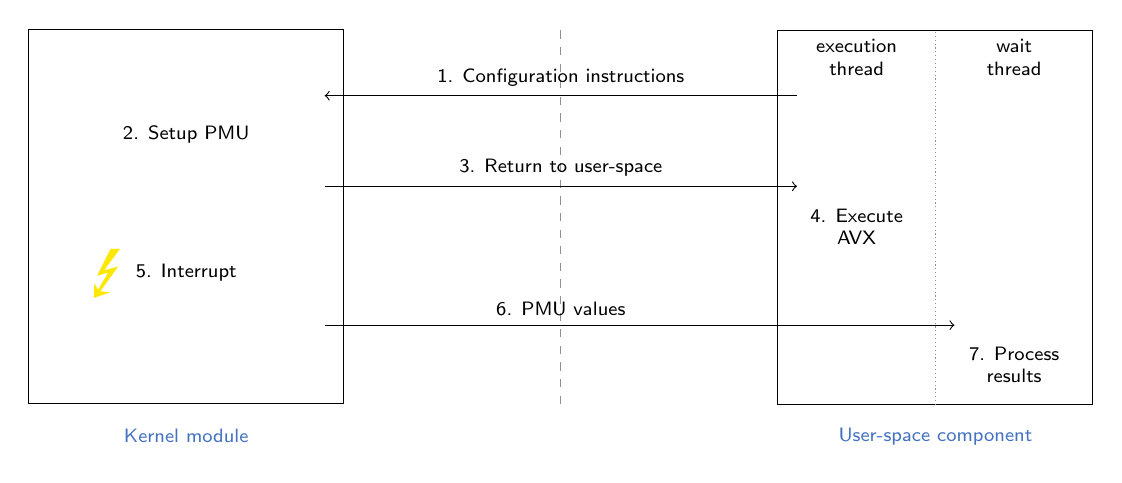
\begin{tikzpicture}[font=\scriptsize]
		\sffamily
		\pgfmathsetmacro{\componentrectwidth}{4}
		\pgfmathsetmacro{\componentrectheight}{4.75}
		\pgfmathsetmacro{\separatordist}{2.75}
		\pgfmathsetmacro{\arrowoverlength}{0.25}
		\pgfmathsetmacro{\arrowlength}{2*(\arrowoverlength + \separatordist)}
		\pgfmathsetmacro{\halfcomponentrectwidth}{\componentrectwidth*0.5}
		\pgfmathsetmacro{\quartercomponentrectwidth}{\componentrectwidth*0.25}

		% kernel
		\draw (0cm,0cm) rectangle ++(\componentrectwidth cm,\componentrectheight) [ref=kernel-rect];
		\node[color=kitblue] at ([yshift=-0.4 cm] kernel-rect south) {Kernel module};
		%\draw[densely dotted] ([yshift=-1cm] kernel-rect north west) -- ++(\componentrectwidth,0) [ref=kernel-sep];
		%\node at ([yshift=-0.5cm] kernel-rect north) {Linux};

		% separator
		\draw[dashed, color=kitdarkgrey] ([xshift=\separatordist cm] kernel-rect south east) -- ([xshift=\separatordist cm] kernel-rect north east) [ref=separator];

		% user-space
		\draw ([xshift=\separatordist cm] separator south east) rectangle ++(\componentrectwidth,\componentrectheight) [ref=user-rect];
		\draw[densely dotted, color=kitdarkgrey] (user-rect south) -- ++(0,\componentrectheight);
		\node[align=center,anchor=north] at ([xshift=-\quartercomponentrectwidth cm] user-rect north) {execution \\ thread};
		\node[align=center,anchor=north] at ([xshift=+\quartercomponentrectwidth cm] user-rect north) {wait \\ thread};
		\node[color=kitblue] at ([yshift=-0.4 cm] user-rect south) {User-space component};

		% steps
		\draw[<-] ([yshift=-0.85cm,xshift=-\arrowoverlength cm] kernel-rect north east) -- ++(\arrowlength,0) node[align=center,pos=.5,above=0] {1. Configuration instructions};
		\node at ([yshift=-1.35cm] kernel-rect north) {2. Setup PMU};
		\draw[->] ([yshift=-2.0cm,xshift=-\arrowoverlength cm] kernel-rect north east) -- ++(\arrowlength,0) node[align=center,pos=.5,above=0] {3. Return to user-space};
		\node[align=center] at ([yshift=-2.5cm,xshift=-\quartercomponentrectwidth cm] user-rect north) {4. Execute \\ AVX};
		\node[color=kityellow] at ([yshift=-3.12cm,xshift=-1cm] kernel-rect north) {\Huge\Lightning};
		\node at ([yshift=-3.1cm] kernel-rect north) {5. Interrupt};
		\draw ([yshift=-3.75cm,xshift=\arrowoverlength cm] user-rect north west) -- ++(-\arrowlength,0) node[align=center,pos=.5,above=0] {6. PMU values};
		\draw[->] ([yshift=-3.75cm,xshift=\arrowoverlength cm] user-rect north west) -- ++(\halfcomponentrectwidth,0);
		\node[align=center] at ([yshift=-4.25cm,xshift=\quartercomponentrectwidth cm] user-rect north) {7. Process \\ results};
	\end{tikzpicture}
	\caption{Simplified analysis framework architecture. The kernel module enables the user-space component to configure the PMU and handles interrupts.}
	\label{fig:analysis:design:overview}
\end{figure*}

\subsection{Kernel Component}
\label{sec:analysis:design:kernel}

Our kernel component is not supposed to conduct any analysis tasks by itself, but is designed to aid the user-space component described later in \Cref{sec:analysis:design:userspace}. We chose to implement it as a module for version~5.1 of the Linux kernel, which implies that it is written in the C programming language. Existence and design of this kernel module are motivated by our user-space component's needs to configure the \gls{PMU} in order to conduct the measurements required for our analysis. This can only be done from kernel-space.

During module startup, the \gls{PMU} is reset to a default state and the performance counter overflow interrupt vector is set in all core's \gls{APIC}'s \glspl{LVT}. Notably, this degrades the functionality of Linux's \texttt{perf} subsystem as \texttt{perf} partially relies on using the \gls{PMU}.

The module interfaces with user-space by defining a device class and then providing a virtual character device of the previously defined class, exposed via \texttt{/dev/reclocking\_analysis} in the virtual file system. User-space may then \texttt{open()} the provided device file and interact with the module by using several offered \texttt{ioctl()} calls.

Execution threads, on the one hand, initiate their execution by using the \texttt{SETUP ioctl()} call. A C \texttt{struct} must be passed that contains a set of \glspl{MSR} to be written by the kernel module -- these are used to configure the \gls{PMU}. In order to increase the precision of our measurements, it is desirable to cut time spent in user-space without actual execution of the code to be measured. Therefore, a value for the \gls{instptr} must also be passed that will be set in the thread's context before returning to user-space, so that the thread will not directly return at the previous position in the \gls{libc}'s \texttt{ioctl()} wrapper but rather be redirected to another location in memory. Optionally, the \texttt{r12}~x86 architectural register may also be set so that the code executed in user-space upon returning is able to access data structures in an easy manner without needing to use the stack. As described further below, the interrupt action must also be defined beforehand by the execution thread. After applying the configuration, the \texttt{ioctl()} handler saves the current \gls{TSC} value and returns to user-space.

Wait threads, one the other hand, start with the \texttt{WAIT\_FOR\_INTERRUPT ioctl()}, which takes a pointer to a \texttt{interrupt\_result} structure in the user-space component where the resulting performance counter values shall be stored later as well as the numeric identifier of a \gls{CPU} core where an interrupt is expected to occur. The calling thread is suspended by setting it into \texttt{TASK\_UNINTERRUPTIBLE} state. This state \cite{kernelschedheader} in Linux's task state machine allows a thread to be woken up only by the kernel itself and not via any user-space mechanisms (e.g., \glspl{UNIXsig}). Consequently, this way we ensure the execution flow is not interrupted unexpectedly.

It is expected that all execution threads that have an associated wait thread trigger a performance counter overflow interrupt some time after setup. The interrupt handler will then proceed with one of multiple actions as instructed by the \texttt{SETUP} call:

\begin{itemize}
	\item \texttt{WAKE\_WAIT\_THREAD}: this action reads all performance counters and writes them along with the current \gls{TSC} value and the recorded \gls{TSC} value at \texttt{SETUP} to the \texttt{interrupt\_result} structure of the corresponding wake wait, which is now waked up from suspension. The execution thread that triggered the interrupt is returned to its previous \acrlong{instptr} (before the \texttt{SETUP} call). Notably, from user-space's view, the original \texttt{SETUP} call returns only now.
	\item \texttt{SET\_MSRS}: this is used for analysis tasks consisting of two consecutive steps. The \gls{TSC} value is recorded and another set of \glspl{MSR} is configured on the thread's core. For the next interrupt, the action is unconditionally set to \texttt{WAKE\_WAIT\_THREAD}.
	\item \texttt{GOTO}: exactly like \texttt{SET\_MSRS}, but also sets a new \acrlong{instptr} on the execution thread.
\end{itemize}

Each of these actions concludes with resetting the \gls{PMU}'s overflow bit and the \gls{APIC}'s state in order to be ready for further interrupts.

A practical software engineering issue arises from the fact that wait threads are suspended in an uninterruptible state after startup: they may easily get stuck due to programming errors that cause a lack of interrupts. For these cases, a third \texttt{ioctl()} call was implemented: \texttt{RESET\_WAIT\_THREADS}, which simply wakes all suspended wait threads and makes their pending \texttt{ioctl()} calls return with an error status.

\subsection{User-Space Component}
\label{sec:analysis:design:userspace}

The user-space component of our analysis framework is the one that implements and performs the actual analysis tasks and is aided by the previously described kernel module by instructing it to configure the \gls{PMU} and handle performance interrupts. Akin to the kernel module, our user-space program is written in C with some additional helper scripts implemented in the PHP scripting language for invocation and monitoring tasks and to generate spreadsheets containing the results. \gls{AVX} instructions included in the program are directly written in x86 assembly.

In order to run tests with different instruction types, an arbitrary number of \gls{ELF} sections containing \gls{AVX} instructions may be included in the component's compiled binary executable. The address of one of these sections and its length must be passed as arguments to the program (these values are easily obtainable using tools like \texttt{objdump}). On startup, one or more executable memory areas, each consisting of four pages, are mapped and filled with the content of the passed section, repeated until the area is full, or alternatively, filled only with a specific amount of repeated instructions. This allows our measurement modes to investigate the \gls{CPU}'s behavior when only a certain amount of \gls{AVX} instructions is executed. In order to ensure the instruction flow does not run outside the allocated area, one of two different loop modes is used at the end of each memory area, depending on the measurement mode:

\begin{itemize}
	\item \texttt{LOOP\_AVX}: a jump instruction to the beginning of the area is added in order to make the constructed code loop -- this allows for infinite \gls{AVX} execution until the executing thread is interrupted.
	\item \texttt{LOOP\_R12\_CMP}: a spinlock-style loop is inserted that constantly compares the value referenced by the pointer stored in the \texttt{r12} register to $0$ and returns as soon as it isn't equal to $0$ anymore:
		\begin{minted}{gas}
		loop:
		cmp 0x0, (%r12)
		je loop
		ret
		\end{minted}
		This way, after some \gls{AVX} instructions were executed, the executor may spin using only scalar instructions until it is instructed to return from outside when another thread updates the value underneath the pointer in \texttt{r12}. Note that our \gls{AVX} memory area does not have its own stack frame in any way, so, assuming that the executing thread jumped into the memory area by using the \texttt{SETUP ioctl()} described in \Cref{sec:analysis:design:kernel}, we actually return the \texttt{ioctl()}'s stack frame here. This is a rather fragile and non-portable approach and may not work as desired with every \gls{libc} implementation.
\end{itemize}

Further, some measurement modes need to execute \gls{AVX} instructions until interrupted and then want to execute purely scalar code to wait for another event. For this purpose, we also allow mapping memory areas that solely consist of an empty loop.

The number of four pages per area was not chosen arbitrarily: on an x86 processor running in \SI{64}{\bit} mode \cite{intelsdmsysprogguide}, pages have a default size of \SI{4}{\kibi\byte}, thus four pages equate a total size of \SI{16}{\kibi\byte}. We originally used an area size of \SI{2}{\mebi\byte} (512 pages), based on the idea of achieving a purely homogeneous workload that does not contain any jumps to increase the precision of our measurements. However, tests showed that the code would become approximately \SI{20}{\percent} faster when run on multiple cores in parallel. We believe this behavior to be caused by instruction cache misses -- although modern \glspl{CPU} commonly feature an \gls{instprefetcher}, there is a caveat: it does not load instructions across page boundaries, and thus, every \SI{4}{\kibi\byte} of instructions we would see a cache miss and a costly pipeline stall until the next instructions arrive from memory. By using parallel execution on multiple cores, this effect is mitigated as the fastest core would already have loaded the instructions into the \gls{L3}, readily available for the other cores. It could be worthwhile to look into huge pages as an alternative solution, though that remains future work.
% TODO is this related to spectre?

As briefly described in \Cref{sec:analysis:design:overview}, the user-space process spawns $n~\in~\mathbb{N}$ execution threads and $w\in\{1,n\}$ wait threads. The value for $n$ is specified as a command line argument, while the amount of wait threads depends on whether \textit{pre-throttling} is enabled. The execution threads are bound to \gls{CPU} cores $1$ to $n$, respectively; the wait threads to the following cores. This also implies that at maximum $\lfloor{}\frac{C}{2}\rfloor{}$ execution threads may be run, where $C$ is the number of \gls{CPU} cores installed in the system, and a minimum of two cores must be available. In pre-throttling mode, the idea is to create an artificial, pre-existing global load situation across several cores. Only results from one core are collected, and thus, only one wait thread is required. The other execution threads start their execution about \SI{150}{\milli\second} earlier than the monitored thread in order to simulate pre-existing load and execute either an infinite (scalar) loop or the same \gls{AVX} code that will also run on the monitored thread, depending on the selection made via the command line. With pre-throttling enabled, it is theoretically possible to have $C-1$ execution threads running. Note that this mode does not have any effect when only one execution thread is used.

In order to avoid inaccuracies caused by preemption, all execution threads use the \texttt{SCHED\_RR} scheduling policy offered by Linux's \gls{CFS} \cite{cfs} which is designed for near-real-time execution and selects real-time threads ordered by their priority; threads of equal priority are executed in a round-robin fashion. \gls{CFS} exposes additional configuration settings \cite{cfsrt} to control the fraction of time that may be consumed by real-time processes, namely \texttt{sched\_rt\_period\_us} and \texttt{sched\_rt\_runtime\_us}. The former sets a time window (\SI{1}{\second} per default) and the latter contains the absolute amount of time within that window that is available to real-time threads (\SI{950}{\milli\second} per default). In theory, we could configure these to allow for infinite real-time execution, however, practical tests have shown this leads to unbearable system hangs that would require further work on our implementation in order to fix. We settled for a value of \SI{990}{\milli\second} for \texttt{sched\_rt\_runtime\_us} as compromise.

In all measurement modes, we configure the following performance events (as documented by Intel in \cite{intelsdmsysprogguide}):

\begin{itemize}
	\item \texttt{CORE\_POWER.LVL0\_TURBO\_LICENSE}: counts core cycles spent in turbo license level 0.
	\item \texttt{CORE\_POWER.LVL1\_TURBO\_LICENSE}: counts core cycles spent in turbo license level 1.
	\item \texttt{CORE\_POWER.LVL2\_TURBO\_LICENSE}: counts core cycles spent in turbo license level 2.
	\item \texttt{CORE\_POWER.THROTTLE}: counts core cycles during which the \gls{OoO} engine is throttled.
	\item \texttt{INT\_MISC.CLEAR\_RESTEER\_CYCLES}: counts core cycles while the execution engine is stalled waiting for instructions to be delivered. This is used to estimate the time spent before the actual execution when switching from kernel-space to user-space in execution threads.
	\item \texttt{FP\_ARITH\_INST\_RETIRED.PACKED}: counts retired packed floating-point \glspl{vectorinst}. Several variants for \SI{128}{\bit}, \SI{256}{\bit} and \SI{512}{bit} vectors and single- and double-precision instructions are available which we select according to the instruction type used in the \gls{AVX} code section passed at startup.
	\item \texttt{UOPS\_DISPATCHED\_PORT.PORT\_0}: counts \glspl{microinst} dispatched by the processor's scheduler at execution port 0. The use of this performance event is motivated by the \textit{Skylake (Server)} microarchitecture the \gls{CPU} we used for our analysis is based on. These processors have an \gls{AVX-512} unit fused from two \SI{256}{\bit} units at ports 0 and 1 \cite{intelxeonscalabledeepdive}. For other microarchitectures, other performance events may be appropriate.
	\item \texttt{UOPS\_DISPATCHED\_PORT.PORT\_5}: counts \glspl{microinst} dispatched by the processor's scheduler at execution port 5. The motivation here is the same as for the performance event counting \glspl{microinst} at port 0, however, only some specific \textit{Skylake (Server)} \glspl{CPU} have an additional, dedicated (i.e., non-fused) \gls{AVX-512} unit at port 5.
\end{itemize}

At startup, wait threads simply block at a synchronization barrier after setting their core affinity. Execution threads, in contrast, need to set their core affinity, the scheduling policy and build up the configuration to pass to the \texttt{SETUP ioctl()} call provided by our kernel module. Afterwards, they block at the same synchronization barrier as the wait threads, unless the thread is used for pre-throttling as described above. As soon as all threads have reached the barrier, the execution threads will enter a \SI{150}{\milli\second} busy-wait loop before calling the \texttt{SETUP ioctl()} to ensure their respective cores are ramped up to their maximum turbo frequency before starting the test run, whereas the wait threads directly jump into the \texttt{WAIT\_FOR\_INTERRUPT ioctl()}.

After execution has completed, there is not much to do for the execution threads: their \texttt{SETUP ioctl()} returns and then they simply exit. Wait threads, on the other side, will again synchronize at a barrier and then output the results as provided by the kernel module one after another before they exit, too. As soon as all threads have completed, the program quits.

\subsection{Measurement Modes}
\label{sec:analysis:design:measurementmodes}

In order to answer the questions named in \Cref{sec:analysis:methodology}, we implemented several different measurement modes in our user-space component, which are to be presented hereafter.

\subsubsection{DOWNCLOCK}
\label{sec:analysis:design:measurementmodes:downclock}

Our first measurement mode is designed to measure the downclocking behavior~--~i.e., how long it takes for a \gls{CPU} to reduce its frequency and whether there is a step to turbo license level~1 before switching to level~2 for instructions that target level~2.

In this mode, we simply map a single memory area with \gls{AVX} code to be run by all execution threads and configure the \gls{PMU} to trigger an interrupt and freeze the performance counters as soon as one cycle is spent in either level~1 or level~2, depending on the target license level passed as command line argument to the program. We use the \texttt{WAKE\_WAIT\_THREAD} interrupt action provided by the kernel component. Thereby, we can measure the time taken for the frequency reduction. When running a test case using this measurement mode with level~2 as target, we will also see whether any cycles were spent in level~1 from the respective performance counter. Thus, this measurement mode indeed answers the aforementioned questions.

\begin{figure*}
	\centering
	\begin{subfigure}[b]{0.5\textwidth}
		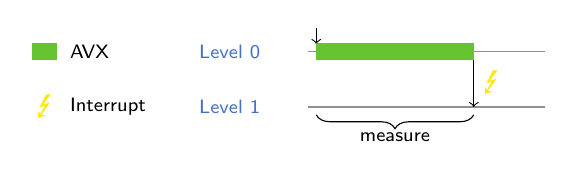
\begin{tikzpicture}[font=\scriptsize]
			\sffamily
			\pgfmathsetmacro{\levelheight}{0.2}
			\pgfmathsetmacro{\linelength}{3}
			\pgfmathsetmacro{\barlength}{0.3}

			% legend
			\draw[fill=kitgreen, color=kitgreen] (-2.5, 0.9) rectangle ++(\barlength cm, \levelheight cm);
			\node[minimum height=\levelheight cm, text centered, anchor=west] at (-2.15, 1) {AVX};

			\node[color=kityellow, align=center] at (-2.35, 0.3) {\large\Lightning};
			\node[minimum height=\levelheight cm, text centered, anchor=west] at (-2.15, 0.3) {Interrupt};

			% level 0
			\node[color=kitblue, minimum height=\levelheight cm, text centered] at (0, 1) {Level~0};
			\draw[color=kitdarkgrey] (1, 1) -- ++(\linelength cm,0);

			% level 1
			\node[color=kitblue, minimum height=\levelheight cm, text centered] at (0, 0.3) {Level~1};
			\draw[color=kitdarkgrey] (1, 0.3) -- ++(\linelength cm,0);

			% bars and transitions
			\draw[<-] (1.1, 1.1) -- ++(0, 0.2);
			\draw[fill=kitgreen, color=kitgreen] (1.1, 0.9) rectangle ++(2cm, \levelheight cm);
			\draw[->, anchor=east] (3.1, 0.9) -- ++(0, -0.6) node[pos=0.5, anchor=west] {\large\color{kityellow}\Lightning};

			\draw[decorate, decoration={brace, amplitude=5pt, mirror}] (1.1, 0.2) -- ++(2cm,0) node[pos=0.5, anchor=north, yshift=-0.1cm] {measure};
		\end{tikzpicture}
		\caption{Level~1}
	\end{subfigure}%
	\begin{subfigure}[b]{0.5\textwidth}
		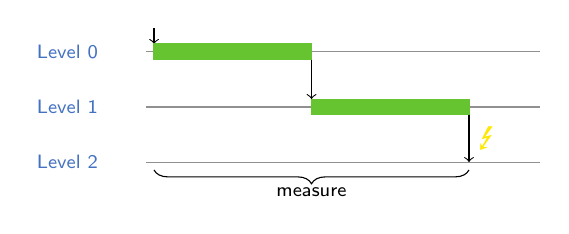
\begin{tikzpicture}[font=\scriptsize]
			\sffamily
			\pgfmathsetmacro{\levelheight}{0.2}
			\pgfmathsetmacro{\linelength}{5}

			% level 0
			\node[color=kitblue, minimum height=\levelheight cm, text centered] at (0, 1) {Level~0};
			\draw[color=kitdarkgrey] (1, 1) -- ++(\linelength cm,0);

			% level 1
			\node[color=kitblue, minimum height=\levelheight cm, text centered] at (0, 0.3) {Level~1};
			\draw[color=kitdarkgrey] (1, 0.3) -- ++(\linelength cm,0);

			% level 2
			\node[color=kitblue, minimum height=\levelheight cm, text centered] at (0, -0.4) {Level~2};
			\draw[color=kitdarkgrey] (1, -0.4) -- ++(\linelength cm,0);

			% bars and transitions
			\draw[<-] (1.1, 1.1) -- ++(0, 0.2);
			\draw[fill=kitgreen, color=kitgreen] (1.1, 0.9) rectangle ++(2cm, \levelheight cm);
			\draw[->, anchor=east] (3.1, 0.9) -- ++(0, -0.5);
			\draw[fill=kitgreen, color=kitgreen] (3.1, 0.2) rectangle ++(2cm, \levelheight cm);
			\draw[->, anchor=east] (5.1, 0.2) -- ++(0, -0.6) node[pos=0.5, anchor=west] {\large\color{kityellow}\Lightning};

			\draw[decorate, decoration={brace, amplitude=5pt, mirror}] (1.1, -0.5) -- ++(4cm,0) node[pos=0.5, anchor=north, yshift=-0.1cm] {measure};
		\end{tikzpicture}
		\caption{Level~2}
	\end{subfigure}
	\caption{Illustration of the \texttt{DOWNCLOCK} measurement mode. This mode measures the time until the requested target license level is reached.}
	\label{fig:analysis:design:measurementmodes:downclock}
\end{figure*}

\subsubsection{UPCLOCK}
\label{sec:analysis:design:measurementmodes:upclock}

After analyzing the downclocking times, the next logical step is to look at the reverse process: the upclocking. Here, we are mainly interested in the time the \gls{CPU} takes before returning back to its non-throttled frequency after the last \gls{AVX} instruction has retired.

Like in the \hyperref[sec:analysis:design:measurementmodes:downclock]{\texttt{DOWNCLOCK}} mode, we map an \gls{AVX} memory area into which the execution threads jump after startup, however, we also map an additional page with an infinite loop. In the first step, we configure an interrupt to be fired after switching to either level~1 or level~2, depending on the input, in order to be able to measure upclocking from both throttle levels. Then, using the \texttt{GOTO} interrupt action, we move the execution thread to the infinite loop page, reset our performance counters and configure an interrupt for when level~0 is reached again and to freeze the performance counters at this point. It is important to not simply leave the core in a completely idle state, as the kernel would then eventually run the \texttt{MWAIT} \cite{intelsdminstructionreference} instruction on the core, causing it to enter a halt state, and thus, our measurements would be useless given that it would not reflect real-world heterogeneous applications, and because the clock is disabled when the core is halted.

Using the described procedure, we measure only the time spent after reaching a turbo license level with reduced frequency until returning to nominal frequency, which is exactly what we are interested in. Notably, in this mode, we instruct the \gls{PMU} to also count cycles while running in kernel-space (i.e., ring~$0$) as this is also time spent without executing \gls{AVX} instructions and thus must be measured to retrieve precise results.

\begin{figure*}
	\centering
	\begin{subfigure}[b]{0.6\textwidth}
		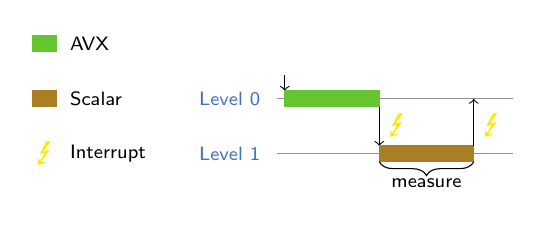
\begin{tikzpicture}[font=\scriptsize]
		\sffamily
		\pgfmathsetmacro{\levelheight}{0.2}
		\pgfmathsetmacro{\linelength}{3}
		\pgfmathsetmacro{\legendbarlength}{0.3}
		\pgfmathsetmacro{\barlength}{1.2}

		% legend
		\draw[fill=kitgreen, color=kitgreen] (-2.5, 1.6) rectangle ++(\legendbarlength cm, \levelheight cm);
		\node[minimum height=\levelheight cm, text centered, anchor=west] at (-2.15, 1.7) {AVX};

		\draw[fill=kitbrown, color=kitbrown] (-2.5, 0.9) rectangle ++(\legendbarlength cm, \levelheight cm);
		\node[minimum height=\levelheight cm, text centered, anchor=west] at (-2.15, 1) {Scalar};

		\node[color=kityellow, align=center] at (-2.35, 0.3) {\large\Lightning};
		\node[minimum height=\levelheight cm, text centered, anchor=west] at (-2.15, 0.3) {Interrupt};

		% level 0
		\node[color=kitblue, minimum height=\levelheight cm, text centered] at (0, 1) {Level~0};
		\draw[color=kitdarkgrey] (0.6, 1) -- ++(\linelength cm,0);

		% level 1
		\node[color=kitblue, minimum height=\levelheight cm, text centered] at (0, 0.3) {Level~1};
		\draw[color=kitdarkgrey] (0.6, 0.3) -- ++(\linelength cm,0);

		% bars and transitions
		\draw[<-] (0.7, 1.1) -- ++(0, 0.2);
		\draw[fill=kitgreen, color=kitgreen] (0.7, 0.9) rectangle ++(\barlength cm, \levelheight cm);
		\draw[->] (1.9, 0.9) -- ++(0, -0.5) node[pos=0.5, anchor=west] {\large\color{kityellow}\Lightning};
		\draw[fill=kitbrown, color=kitbrown] (1.9, 0.2) rectangle ++(\barlength cm, \levelheight cm);
		\draw[->] (3.1, 0.4) -- ++(0, 0.6) node[pos=0.41666, anchor=west] {\large\color{kityellow}\Lightning};

		\draw[decorate, decoration={brace, amplitude=5pt, mirror}] (1.9, 0.2) -- ++(\barlength cm,0) node[pos=0.5, anchor=north, yshift=-0.1cm] {measure};
		\end{tikzpicture}
		\caption{Level~1}
	\end{subfigure}%
	\begin{subfigure}[b]{0.4\textwidth}
		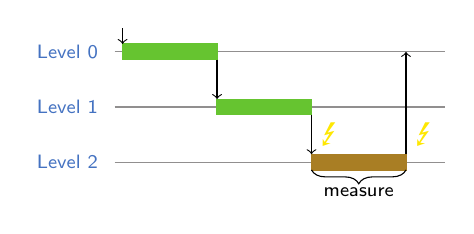
\begin{tikzpicture}[font=\scriptsize]
		\sffamily
		\pgfmathsetmacro{\linelength}{4.2}
		\pgfmathsetmacro{\barlength}{1.2}
		\pgfmathsetmacro{\barheight}{0.2}
		\pgfmathsetmacro{\linemargin}{0.6}
		\pgfmathsetmacro{\linepadding}{0.1}
		\pgfmathsetmacro{\linedistance}{0.7}
		\pgfmathsetmacro{\linezeroy}{1}
		\pgfmathsetmacro{\lineoney}{\linezeroy-\linedistance}
		\pgfmathsetmacro{\linetwoy}{\lineoney-\linedistance}
		\pgfmathsetmacro{\interbararrowheight}{\linedistance-\barheight}
		\pgfmathsetmacro{\measurey}{\linetwoy-0.5*\barheight}

		% level 0
		\node[color=kitblue, minimum height=\barheight cm, text centered] at (0, \linezeroy) {Level~0};
		\draw[color=kitdarkgrey] (\linemargin, \linezeroy) -- ++(\linelength cm,0);

		% level 1
		\node[color=kitblue, minimum height=\barheight cm, text centered] at (0, \lineoney) {Level~1};
		\draw[color=kitdarkgrey] (\linemargin, \lineoney) -- ++(\linelength cm,0);

		% level 2
		\node[color=kitblue, minimum height=\barheight cm, text centered] at (0, \linetwoy) {Level~2};
		\draw[color=kitdarkgrey] (\linemargin, \linetwoy) -- ++(\linelength cm,0);

		% bars and transitions
		\pgfmathsetmacro{\baronex}{\linemargin+\linepadding}
		\pgfmathsetmacro{\baroney}{\linezeroy-0.5*\barheight}
		\draw[fill=kitgreen, color=kitgreen] (\baronex, \baroney) rectangle ++(\barlength cm, \barheight cm);

		\pgfmathsetmacro{\bartwox}{\baronex+\barlength}
		\pgfmathsetmacro{\bartwoy}{\lineoney-0.5*\barheight}
		\draw[fill=kitgreen, color=kitgreen] (\bartwox, \bartwoy) rectangle ++(\barlength cm, \barheight cm);

		\pgfmathsetmacro{\barthreex}{\bartwox+\barlength}
		\pgfmathsetmacro{\barthreey}{\linetwoy-0.5*\barheight}
		\draw[fill=kitbrown, color=kitbrown] (\barthreex, \barthreey) rectangle ++(\barlength cm, \barheight cm);

		\pgfmathsetmacro{\arrowoney}{\baroney+\barheight}
		\draw[<-] (\baronex, \arrowoney) -- ++(0, 0.2);

		\draw[->, anchor=east] (\bartwox, \baroney) -- ++(0, -\interbararrowheight cm);

		\draw[->, anchor=east] (\barthreex, \bartwoy) -- ++(0, -\interbararrowheight cm) node[pos=0.5, anchor=west] {\large\color{kityellow}\Lightning};

		\pgfmathsetmacro{\arrowfourx}{\barthreex+\barlength}
		\pgfmathsetmacro{\arrowfoury}{\barthreey+\barheight}
		\pgfmathsetmacro{\arrowfourlength}{\interbararrowheight+0.5*\barheight+\linedistance}
		\pgfmathsetmacro{\arrowfournodepos}{0.5*\interbararrowheight/\arrowfourlength}
		\draw[->, anchor=east] (\arrowfourx,\arrowfoury) -- ++(0, \arrowfourlength cm) node[pos=\arrowfournodepos, anchor=west] {\large\color{kityellow}\Lightning};

		\draw[decorate, decoration={brace, amplitude=5pt, mirror}] (\barthreex, \measurey) -- ++(\barlength cm,0) node[pos=0.5, anchor=north, yshift=-0.1cm] {measure};
		\end{tikzpicture}
		\caption{Level~2}
	\end{subfigure}
	\caption{The \texttt{UPCLOCK} mode measures how long it takes a core to return to its level~0 frequency after an \gls{AVX}-induced reduction.}
	\label{fig:analysis:design:measurementmodes:upclock}
\end{figure*}

\subsubsection{PRE\_THROTTLE\_TIME}
\label{sec:analysis:design:measurementmodes:prethrottlethroughput}

As cited at the beginning of \hyperref[sec:analysis]{this chapter}, Intel talks in their optimization manual \cite{inteloptimizationmanual} about the \glspl{CPU} operating at a \enquote{lower peak capability} before the switch to a turbo license level with lower frequency is completed. Early experimentation showed this state is seemingly represented by the \texttt{CORE\_POWER.THROTTLE} performance event which is described \cite{intelsdmsysprogguide} to count cycles where the \gls{OoO} engine is throttled. We want to find out when exactly this throttle state is activated and what instruction throughput the \gls{CPU} achieves before throttling to get an idea of the theoretically possible performance if the frequency reduction did not exist.

For this purpose, the \texttt{PRE\_THROTTLE\_TIME} mode conceptually works very much the same way as the \hyperref[sec:analysis:design:measurementmodes:downclock]{\texttt{DOWNCLOCK}} mode: we configure an interrupt that fires and freezes the performance counters as soon as the first cycle was spent in throttled mode and run our \gls{AVX} code using the \texttt{WAIT\_FOR\_INTERRUPT} interrupt action. Thereby, we obtain the desired information about the behavior during the time between starting execution and \gls{OoO} engine throttling.

\begin{figure*}
	\centering
	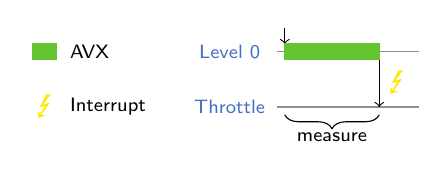
\begin{tikzpicture}[font=\scriptsize]
		\sffamily
		\pgfmathsetmacro{\levelheight}{0.2}
		\pgfmathsetmacro{\linelength}{1.8}
		\pgfmathsetmacro{\legendbarlength}{0.3}
		\pgfmathsetmacro{\barlength}{1.2}

		% legend
		\draw[fill=kitgreen, color=kitgreen] (-2.5, 0.9) rectangle ++(\legendbarlength cm, \levelheight cm);
		\node[minimum height=\levelheight cm, text centered, anchor=west] at (-2.15, 1) {AVX};

		\node[color=kityellow, align=center] at (-2.35, 0.3) {\large\Lightning};
		\node[minimum height=\levelheight cm, text centered, anchor=west] at (-2.15, 0.3) {Interrupt};

		% level 0
		\node[color=kitblue, minimum height=\levelheight cm, text centered] at (0, 1) {Level~0};
		\draw[color=kitdarkgrey] (0.6, 1) -- ++(\linelength cm,0);

		% throttle
		\node[color=kitblue, minimum height=\levelheight cm, text centered] at (0, 0.3) {Throttle};
		\draw[color=kitdarkgrey] (0.6, 0.3) -- ++(\linelength cm,0);

		% bars and transitions
		\draw[<-] (0.7, 1.1) -- ++(0, 0.2);
		\draw[fill=kitgreen, color=kitgreen] (0.7, 0.9) rectangle ++(\barlength cm, \levelheight cm);
		\draw[->] (1.9, 0.9) -- ++(0, -0.6) node[pos=0.5, anchor=west] {\large\color{kityellow}\Lightning};

		\draw[decorate, decoration={brace, amplitude=5pt, mirror}] (0.7, 0.2) -- ++(\barlength cm,0) node[pos=0.5, anchor=north, yshift=-0.1cm] {measure};
	\end{tikzpicture}
	\caption{After starting to execute heavy \gls{AVX} instructions, a core enters a state where the \gls{OoO} engine is throttled. The \texttt{PRE\_THROTTLE\_TIME} mode measures the time it takes until the throttling takes place.}
	\label{fig:analysis:design:measurementmodes:prethrottlethroughput}
\end{figure*}

\subsubsection{REQUIRED\_INSTRUCTIONS}
\label{sec:analysis:design:measurementmodes:nonavxtime}

To obtain a model of the reclocking algorithm that is as complete as possible, we are not only interested in the time it takes for a \gls{CPU} to switch turbo license levels, but also how many instructions are precisely required to eventually trigger the frequency reduction.

The implementation of this measurement mode is more complex compared to the other modes and also partially depends on the license level transition to be examined. For this mode, the idea is to run multiple iterations where the amount of \gls{AVX} instructions is increased in every iteration until executing the code triggers an interrupt due to a license level switch within a reasonable amount of time.

In every case, we map an \gls{AVX} memory area in \texttt{LOOP\_R12\_CMP} mode which initially contains only just one copy of the \gls{AVX} code in the selected \gls{ELF} section. When license level~2 was chosen as target, we additionally map an area in \texttt{LOOP\_AVX} mode that is executed until level~1 is reached. In \gls{AVX} pre-throttling mode, another area is created in \texttt{LOOP\_AVX} mode to be run by execution threads used for pre-throttling.

In case level~1 is targeted, all (non-pre-throttling) execution threads directly jump into the \texttt{LOOP\_R12\_CMP} area and use the \texttt{WAKE\_WAIT\_THREAD} interrupt action mode. For level~2 as target, we select the \texttt{GOTO} interrupt action and first jump into the aforementioned \texttt{LOOP\_AVX} area and configure an interrupt to be triggered as soon as one cycle in level~1 was completed. Afterwards, the execution threads are also moved to the \texttt{LOOP\_R12\_CMP}. In our \texttt{SETUP} configuration, we instruct our kernel module to fill the \texttt{r12} register with a pointer to a global \texttt{try\_elapsed} variable defined in the program so that the loop in the executed code returns as soon as \texttt{try\_elapsed} is set.

While the execution threads are running, our main thread awaits a \SI{1}{\milli\second} delay and then checks whether an interrupt was triggered on all expected cores. If yes, the test run has completed and the program quits. Otherwise, we exit all execution threads by setting \texttt{try\_elapsed} and then remap the \texttt{LOOP\_R12\_CMP} with one more copy of the \gls{AVX} code than in the previous iteration. Wait threads that completed because an interrupt was triggered on their corresponding execution thread are respawned, afterwards we reset \texttt{try\_elapsed} and start the execution threads again. Unlike in the first iteration, where execution threads generally spin for \SI{150}{\milli\second} to ramp up the core frequency (as described in \Cref{sec:analysis:design:userspace}), we only have them spin for \SI{3}{\milli\second} now as their respective cores are already running at the desired frequency but possibly need to return from an attained turbo license level. This procedure repeats until we have enough \gls{AVX} code in our mapped area to trigger interrupts on all desired cores.

At the end, the number of copies of the \gls{AVX} code in the \texttt{LOOP\_R12\_CMP} area reflects the amount of instructions needed to cause the frequency transition.

\section{Results}
\label{sec:analysis:results}

We use the described analysis framework to conduct measurements with several different \gls{AVX} instructions using all available combinations of modes, i.e., with and without pre-throttling, different target turbo license levels, with turbo frequencies enabled and disabled and with all possible amounts of cores enabled. All measurements are executed 1000 times in order to obtain statistical certainty. In this section, we present our system setup, describe the precise instructions we used for testing and present as well as discuss the results.

\subsection{System Setup}
\label{sec:analysis:results:systemsetup}

To execute our analysis tasks, we used an Intel Core i9-7940X processor which features 14 physical cores with twofold \gls{SMT} running at a nominal base frequency of \SI{3.1}{\giga\hertz} with a maximum turbo frequency of \SI{4.3}{\giga\hertz} \cite{intel7940x}. Additionally, the chip supports \textit{Intel Turbo Boost Max Technology 3.0}, essentially meaning that two cores may operate at a higher turbo frequency, namely \SI{4.4}{\giga\hertz}. These cores are selected based on their electrical and thermal properties during the manufacturing process \cite{intelxeonscalabledeepdive} -- this technique is otherwise also known as \textit{speed binning} \cite{lopata2012speed}. The chip's nominal \gls{TDP} is specified at \SI{165}{\watt}, and as such, this is the maximum power consumption the chip will sustain over long time periods.

This \gls{CPU} is based on the \textit{Skylake (Server)} microarchitecture, the first x86 implementation featuring support for the \gls{AVX-512} extension \cite{intelxeonscalabledeepdive}, making it one of the oldest processors that expose the \gls{AVX} reclocking issue for heterogeneous workloads. However, not all \glspl{CPU} built with this microarchitecture feature the same amount of \SI{512}{\bit}-vector execution units: some have two, others only one. The i9-7940X used here has two.

The processor was equipped on an ASUS TUF X299 MARK 2 motherboard along with \SI{32}{\gibi\byte} of DDR4 system memory operating at a frequency of \SI{2666}{\mega\hertz} and a \gls{NVMe} Solid State Drive. The motherboard was not chosen arbitrarily: being designed for the needs of the overclocking community, it -- unlike most other motherboards for this platform -- allows to customize the frequency targets for \gls{AVX}-induced reclocking in its \gls{UEFI}'s configuration menu. For this analysis, the offsets were configured to 3 and 7 for turbo license levels 1 and 2, respectively, resulting in target frequencies of \SI{3.4}{\giga\hertz} and \SI{2.8}{\giga\hertz}.

We opted to use Fedora 29 (Server Edition) as operating system with a custom-built Linux 5.1.0 kernel and glibc version 2.28-33. The kernel and all of our own code were compiled using GCC 8.3.1-2 with the default \texttt{-O2} optimization level.

In order to minimize overhead and latencies caused by context switches from user-space to kernel-space and vice versa, we disabled all mitigations provided by the Linux kernel for hardware vulnerabilities found in recent \glspl{CPU} (e.g., \textsc{Spectre} and \textsc{Meltdown}) as well as \gls{KASLR}.

\subsection{Tested Instructions}
\label{sec:analysis:results:testedinstructions}

In order to create a precise model of the \gls{AVX} reclocking algorithm as it was implemented by Intel, we want to conduct our measurements with different kinds of \gls{AVX} instructions to find possible differences in the behavior. Note that we only tested homogeneous loads and did not run any tests with heterogeneous mixtures of different instruction classes. This remains as future work.

We tried to select both floating-point and integer operations that reflect the \enquote{heavy} and \enquote{light} instruction types as defined in Intel's optimization manual \cite{inteloptimizationmanual} as well as instructions we guess to be implemented differently in the hardware's execution units. Consequently, we chose the following subset of \gls{AVX} instructions for our measurements (as obtained from Intel's manual for software developers \cite{intelsdminstructionreference}):

\begin{itemize}
	\item \texttt{vfmaddsub132pd} (double-precision) and \texttt{vfmaddsub132ps} (single-precision): these are floating-point \gls{FMA} instructions that alternatingly add and subtract the values from a third vector after multiplying the values from two other vectors. I.e., for input vectors $a$, $b$ and $c$, they calculate the result vector $r$ according to the following rule:
	\begin{displaymath}
		\begin{pmatrix}
		r_1 \\
		r_2 \\
		r_3 \\
		\dots
		\end{pmatrix}
		\coloneqq
		\begin{pmatrix}
		a_1 * b_1 + c_1 \\
		a_2 * b_2 - c_2 \\
		a_3 * b_3 + c_3 \\
		\dots
		\end{pmatrix}
	\end{displaymath}
	\item \texttt{vmulpd} (double-precision) and \texttt{vmulps} (single-precision): those instructions simply calculate the products of all corresponding floating-point members from two input vectors.
	\item \texttt{vpmullq}: multiplies corresponding \SI{64}{\bit} integers from two input vectors into \SI{128}{\bit} intermediate results and stores the lower \SI{64}{\bit}s of each in the target result vector.
	\item \texttt{vpackssdw}: this instruction merges two vectors with signed \SI{32}{\bit} integers into one vector consisting of signed \SI{16}{\bit} integers by handling overflow conditions via saturation arithmetic, i.e., for values larger than $32767$ ($=2^{15}-1$) or smaller than $-32768$ ($=-2^{15}$), the conversion results in these extreme values. In mathematical terms, the operation may be described as follows for input vectors $a$, $b$ and result vector $r$:
		\begin{displaymath}
		\forall i \in \{1,\dots,|a|\} \cap \mathbb{N}\colon r_i \coloneqq saturate(a_i), r_{|a|+i} \coloneqq saturate(b_i)
		\end{displaymath}
		where $saturate$ is defined as
		\begin{displaymath}
		saturate\colon
		\begin{cases}
			\{-2^{31}, \dots, 2^{31}-1\} \cap \mathbb{Z} \longrightarrow \{-2^{15}, \dots, 2^{15}-1\} \cap \mathbb{Z}, \\
			x \mapsto min(2^{15}-1, max(x, -2^{15})).
		\end{cases}
		\end{displaymath}
		Note that $|a| = |b|$ and $|r| = |a| + |b|$.
	\item \texttt{vpaddsw}: adds signed \SI{16}{\bit} integers from two input vectors using saturation arithmetic as described above.
	\item \texttt{vpmaddwd}: an \gls{FMA}-style operation that first multiplies corresponding signed \SI{16}{\bit} integers from two input vectors, thereby creating an equal amount of \SI{32}{\bit} temporary results. Afterwards, the adjacent results are added together to generate the result vector. For input vectors $a$ and $b$, this is the operation executed to obtain the result vector $r$:
		\begin{displaymath}
		\begin{pmatrix}
		r_1 \\
		r_2 \\
		\dots
		\end{pmatrix}
		\coloneqq
		\begin{pmatrix}
		(a_1*b_1) + (a_2*b_2) \\
		(a_3*b_3) + (a_4*b_4) \\
		\dots
		\end{pmatrix}
		\end{displaymath}
\end{itemize}

We wrote \gls{ELF} sections for our user-space component (as described in \Cref{sec:analysis:design:userspace}) containing assembly code for all of these instructions in two variants with \SI{256}{\bit} \texttt{YMM} and \SI{512}{\bit} \texttt{ZMM} registers, respectively. Additionally, for each variant, there are two versions: an \enquote{unrolled} one and another non-\enquote{unrolled} version. The non-unrolled ones simply contain a single instruction using the first three registers, e.g.:

\begin{center}
	\begin{minted}{gas}
	vfmaddsub132pd %zmm0, %zmm1, %zmm2
	\end{minted}
\end{center}

By constantly keeping to execute the same instruction with the same operands, we create some artificial register pressure that prevents a core's scheduler from maximizing utilization of the two \SI{512}{\bit}-vector units available in the execution engine. The unrolled versions, on the other side, alleviate this pressure by repeating the same instruction, but with different register operands:

\begin{center}
	\begin{minted}{gas}
	vfmaddsub132pd %zmm0, %zmm0, %zmm1
	vfmaddsub132pd %zmm0, %zmm0, %zmm2
	vfmaddsub132pd %zmm0, %zmm0, %zmm3
	...
	\end{minted}
\end{center}

Every unrolled section contains the same instruction repeated 31 times, always using \texttt{\%zmm0}/\texttt{\%ymm0} for the first two operands and \texttt{\%zmm\{1-31\}}/\texttt{\%ymm\{1-31\}} as last operand, thereby, we exhaustively make use of all 32 \texttt{ZMM}/\texttt{YMM} architectural registers available on \gls{AVX-512}-capable processors.

\subsection{Downclocking}
\label{sec:analysis:results:downclocking}

For our model of Intel's \gls{AVX} reclocking algorithm, the downclocking behavior -- i.e., the process of frequency reduction when executing \gls{AVX} instructions -- is an important puzzle piece. Here, we want to answer questions such as \enquote{How long does it take a \gls{CPU} to switch to its reduced frequency?} and \enquote{When is a frequency reduction triggered?}. We obtained the results to be presented in this section using the \hyperref[sec:analysis:design:measurementmodes:downclock]{\texttt{DOWNCLOCK}}, \hyperref[sec:analysis:design:measurementmodes:prethrottlethroughput]{\texttt{PRE\_THROTTLE\_TIME}} and \hyperref[sec:analysis:design:measurementmodes:nonavxtime]{\texttt{REQUIRED\_INSTRUCTIONS}} modes provided by our measurement system as described in \Cref{sec:analysis:design}.

Coarsely, we found the \gls{CPU} to generally run through the following steps for its frequency reduction:

\begin{enumerate}
	\item Throttle the \acrlong{OoO} engine
	\item Switch to turbo license level 1 and alleviate \gls{OoO} engine throttling
	\item Switch to turbo license level 2 (for \gls{AVX-512} \enquote{heavy} instructions)
\end{enumerate}

This already contains our first insight: even for \gls{AVX-512} instructions that Intel defines to be \enquote{heavy}, the processor will first switch to license level~1 and spend some time in that mode before performing another frequency shift to level~2 -- Intel does not mention this in their optimization manual \cite{inteloptimizationmanual}. This information is easily obtained by executing the \hyperref[sec:analysis:design:measurementmodes:downclock]{\texttt{DOWNCLOCK}} mode twice with both levels as targets -- if the \glspl{CPU} did not make this intermediate step, the test would simply hang when executed with level~1 as target as this level would never be reached.

Similarly, we can reach another interesting insight: even \gls{AVX-512} heavy instructions do not always trigger a switch to level~2. We observed this behavior with the \texttt{vfmaddsub132pd} instruction, for which only the unrolled version (i.e., the one without register pressure) will ever reach level~2. The very same behavior exists with the \SI{256}{\bit} version of this instruction, too: the core only switches to level~1 when unrolled.

We can imagine two different factors that could potentially influence this decision: the load on the core's \gls{AVX} units and the register pressure itself.

\begin{figure}
	\begin{tikzpicture}[trim axis left]
	\sffamily
	\begin{axis}[
		xlabel={Runs ($n=1000$)},
		ylabel={Instructions per Cycle},
		scale only axis,
		width=\textwidth,
		height=5cm,
		axis lines=left,
		ymin=0,
		ymax=0.45,
		xtick=\empty,
		xmin=-10,
		xmax=1010
	]
		\addplot[only marks, color=kitgreen] table {plots/avx_dp_fma_512_l1_1cpus_downclock_throughput.csv} node[pos=0.5,below=0.25cm] {non-unrolled};
		\addplot[only marks, color=kitblue] table {plots/avx_dp_fma_512_unrolled_l1_1cpus_downclock_throughput.csv} node[pos=0.5,below=0.6cm] {unrolled};
	\end{axis}
	\end{tikzpicture}
	\caption{Throughput of the \texttt{vfmaddsub132pd} instruction before switching from level~0 to level~1 is doubled when unrolled.}
	\label{fig:analysis:results:downclocking:avx_dp_fma_512_unrolled_l1_1cpus_downclock+avx_dp_fma_512_l1_1cpus_downclock:throughput}
\end{figure}

Before the first frequency reduction from level~0 to level~1 happens, we find that the instruction throughput (\gls{IPC}) of the \SI{512}{\bit} variant is precisely doubled from $0.21$ to $0.42$ on average with the unrolled version compared to the non-unrolled implementation, as depicted in \Cref{fig:analysis:results:downclocking:avx_dp_fma_512_unrolled_l1_1cpus_downclock+avx_dp_fma_512_l1_1cpus_downclock:throughput}.

This is expected: as described in \Cref{sec:analysis:results:testedinstructions}, the \gls{CPU} we used for our tests features two \gls{AVX-512} units per core, and as such, when no register pressure prevents a core from paralleling consecutive instructions, it can make full utilization of both units. However, we also found that the cores always run roughly equal amounts of instructions through both units, even in the non-unrolled case. Most likely, Intel's scheduler uses a simple round-robin algorithm to assign \glspl{microinst} to the units. This is a sign that the load on the units is not the determining factor: in the non-unrolled case the units take turns and each one stays unloaded only for a few cycles at a time.

On the other side, the theory of the register pressure being the culprit here is supported by a patent on local power gating in processors published by Intel \cite{bonen2016performing}: here, Intel describes a technique to dynamically cut and restore power to both vector units and vector registers upon demand to save energy, which is likely implemented in our system's processor as described. Notably, these are controlled independent of each other and it is also noted that the \texttt{vzeroupper} instruction directly impacts the power gating behavior. This instruction zeroes the upper \SI{384}{\bit}s of each architectural \SI{512}{\bit} vector register \cite{intelsdminstructionreference}. Indeed, if we explicitly set the \SI{512}{\bit} register \texttt{ZMM0} to a value before starting execution, we find that heavy \SI{256}{\bit} (i.e., \gls{AVX2}) vector instructions -- which would normally only cause switches to level~1 -- suddenly trigger frequency switches to level~2, too, but not anymore if we additionally execute \texttt{vzeroupper} after setting \texttt{ZMM0}. This is not documented in Intel's description of the reclocking algorithm, but hints that the register usage directly impacts the turbo license level selection in addition to the types of the executed instructions.

Apart from this discrepancy, we found that Intel's description of the instruction types and their associated turbo license levels holds true for the instructions we selected for testing. Now that we know the steps for frequency reductions, the next logical step is to find out when each of them occurs, what is required to trigger them and how much time a core spends in each state.

In \Cref{sec:analysis:design:measurementmodes:prethrottlethroughput}, we described the implementation of the \texttt{PRE\_THROTTLE\_TIME} measurement mode, designed to find out how long \gls{AVX} instructions may be executed before the \acrlong{OoO} engine is throttled with the added bonus of being able to measure what throughput could theoretically be achieved if there was no frequency reduction at all.

The answer here, however, is very simple: in all tested cases, the throttling occurs immediately after execution of the first instruction has completed -- no matter what instruction is tested, how many cores are used or whether pre-throttling is enabled. This also means that we are unable to measure the theoretically achievable throughput here: with a duration of just one instruction, no reliable numbers may be obtained.

Next, we are interested in the amount of instructions required to eventually trigger a switch to level~1. This is what the \hyperref[sec:analysis:design:measurementmodes:nonavxtime]{\texttt{REQUIRED\_INSTRUCTIONS}} measurement mode was built for: it incrementally builds and executes \gls{AVX} code with more instructions until a license level switch can be observed within a time window after an execution iteration.

Here, we indeed found interesting differences between different instruction types: all \SI{512}{\bit} ones require just exactly one instruction to be executed and the core is going to switch to level~1. For \SI{256}{\bit} instructions, however, a quite different picture emerges: \Cref{fig:analysis:results:downclocking:avx_dp_fma_256_unrolled_l1_1cpus_non_avx_time:avx_instructions} depicts the required amount of instructions exemplary for the \SI{256}{\bit} \texttt{vfmaddsub132pd} unrolled case, without pre-throttling and with one core. The result varies between a minimum of $3317$ and a maximum of $30845$ instructions while the average and the median are set rather near each other, at $12982.8$ and $12431$, respectively. \Cref{fig:analysis:results:downclocking:avx_dp_fma_256_unrolled_l1_1cpus_non_avx_time:avx_instructions:histogram} shows the same data, plotted as a histogram. It becomes clearly visible that the median is far nearer to the minimum than it is to the maximum.

\begin{figure}
	\begin{tikzpicture}[trim axis left]
	\sffamily
	\begin{axis}[
		xlabel={Runs ($n=1000$)},
		ylabel={Instructions},
		scale only axis,
		width=\textwidth,
		height=5cm,
		axis lines=left,
		ymin=1700,
		ymax=32000,
		xtick=\empty,
		xmin=-10,
		xmax=1010,
		axis y discontinuity=parallel
	]
		\addplot[only marks, color=kitblue] table {plots/avx_dp_fma_256_unrolled_l1_1cpus_non_avx_time_avx_instructions.csv};
	\end{axis}
	\end{tikzpicture}
	\caption{Required \SI{256}{\bit} \texttt{vfmaddsub132pd} instructions to trigger a turbo license switch to level~1. Unlike with \SI{512}{\bit} instructions, the amount varies a lot.}
	\label{fig:analysis:results:downclocking:avx_dp_fma_256_unrolled_l1_1cpus_non_avx_time:avx_instructions}
\end{figure}

\begin{figure}
	\begin{tikzpicture}[trim axis left]
	\sffamily
	\begin{axis}[
		ybar,
		ymin=0,
		xlabel={Instructions},
		scale only axis,
		width=\textwidth,
		height=5cm,
		axis lines=left,
		xmin=2900,
		xmax=32000,
		ymax=245
	]
		\addplot[color=kitblue, fill=kitblue, hist] table {plots/avx_dp_fma_256_unrolled_l1_1cpus_non_avx_time_avx_instructions.csv};
		\draw[color=kitgreen, thick] ({axis cs:12431,0}) -- ({axis cs:12431,238}) node[anchor=west, pos=0.96] {median = 12431};
	\end{axis}
%	\begin{axis}[
%		axis y line=none,
%		axis x line=none,
%		scale only axis,
%		width=\textwidth,
%		height=5cm,
%		xmin=2900,
%		xmax=32000
%	]
%		\addplot[color=kitgreen, domain=2900:32000, smooth, thick] {x^(6.6985-1)/((1938.2)^(6.6985)*(6.6985)!)*exp(-x/1938.2)};
%	\end{axis}
	\end{tikzpicture}
	\caption{Histogram of the data depicted in \Cref{fig:analysis:results:downclocking:avx_dp_fma_256_unrolled_l1_1cpus_non_avx_time:avx_instructions}. The distance between median and maximum is much larger than between median and minimum.}
	\label{fig:analysis:results:downclocking:avx_dp_fma_256_unrolled_l1_1cpus_non_avx_time:avx_instructions:histogram}
\end{figure}

We find that average and median values rise when executing the test with more cores. While this may seem surprising at first glance, it is expected: when run with multiple cores, the test only ends if a frequency switch is triggered on all cores. Therefore, given the high variance of the results, it becomes less likely that all cores reach a frequency switch with less instructions.

While pre-throttling does not seem to have any effect that can not be attributed to statistical noise, disabling turbo frequencies does have one: we can still observe a high variance within the results, but all statistic measures are \emph{lower}: with a single core, we find a minimum of $527$, a maximum of $21793$, $8642.49$ on average, and a median of $8137.5$. This is intriguing as one would expect a frequency drop to be less necessary when starting off a lower base frequency. We can not be sure of an explanation for this, however, this observation may hint that voltage stability is a crucial factor here: in the previously cited patent \cite{bonen2016performing}, Intel notes that a voltage drop may occur due to rising electrical resistance upon powering the vector units and that a detector for this situation is in place. Given that, at a lower frequency, the core also runs at a lower voltage, it seems plausible that the voltage drops below the critical threshold earlier as the added resistance is the same.
% todo this theory may be verified by testing different chips of the same model and perhaps also applying higher Vcore

With these results we have fully established all conditions required for \gls{AVX}-induced frequency reductions to level~1, now we are interested in the time required for the actual switch.

\begin{figure}
	\begin{tikzpicture}[trim axis left]
	\sffamily
	\begin{axis}[
		xlabel={Runs ($n=1000$)},
		ylabel={\si{\micro\second}},
		scale only axis,
		width=\textwidth,
		height=5cm,
		axis lines=left,
		ymin=15,
		ymax=50,
		xtick=\empty,
		xmin=-10,
		xmax=1010,
		axis y discontinuity=parallel
	]
	\addplot[only marks, color=kitblue] table {plots/avx_dp_fma_512_l1_1cpus_downclock_time.csv};
	\end{axis}
	\begin{axis}[
		ylabel={\si{\micro\second}},
		scale only axis,
		width=\textwidth,
		height=5cm,
		hide axis,
		ymin=15,
		ymax=50,
		xtick=\empty,
		xmin=0,
		xmax=1000
	]
	\addplot[color=kitgreen, domain=0:1000, thick] {24.593225806452} node[pos=0, below=0.7cm, anchor=west] {median = \SI{24.59}{\micro\second}};
	\end{axis}
	\end{tikzpicture}
	\caption{Downclocking time to level~1 for the \SI{512}{\bit} \texttt{vfmaddsub132pd} instruction. The results are very homogeneous around a median of \SI{24.59}{\micro\second}.}
	\label{fig:analysis:results:downclocking:avx_dp_fma_512_l1_1cpus_downclock:time}
\end{figure}

Again, we find \SI{512}{\bit} and \SI{256}{\bit} instructions to have noticeable differences. For example, with \SI{512}{\bit} \texttt{vfmaddsub132pd} instructions executed on a single core, all results are very homogeneously distributed around a median of \SI{24.59}{\micro\second} with only a few outliers, as depicted in \Cref{fig:analysis:results:downclocking:avx_dp_fma_512_l1_1cpus_downclock:time}. There is no statistically relevant difference with other \SI{512}{\bit} instructions, however, median and deviation both rise with multiple cores: exemplarily looking at three cores (\Cref{fig:analysis:results:downclocking:avx_dp_fma_512_l1_3cpus_downclock:time}), we find the average of the median across all three cores to be at \SI{27.39}{\micro\second} -- an increase of nearly three microseconds. While the standard deviation with only one core is very low at $0.0025$, it quintuples with three cores and amounts to an average of $0.013$. Notably, this increase only happens with pre-throttling disabled. This is interesting because it tells us that the frequency is not the determining factor here: the maximum turbo frequency of a single core depends on the available electrical power budget as well as on how many cores are under load, and thus, with three cores compared to only one, each core runs at a lower frequency. If, however, the increase is not visible with pre-throttling -- i.e., when two cores are already at level~1 -- the lower frequency can not be at fault for the increased latency. A simple and plausible explanation could be that the \gls{PCU} requires more time to make its decision when more license requests are pending.

\begin{figure}
	\begin{tikzpicture}[trim axis left]
	\sffamily
	\begin{axis}[
		xlabel={Runs ($n=1000$)},
		ylabel={\si{\micro\second}},
		scale only axis,
		width=\textwidth,
		height=5cm,
		axis lines=left,
		ymin=15,
		ymax=50,
		xtick=\empty,
		xmin=-10,
		xmax=1010,
		axis y discontinuity=parallel
	]
	\addplot[only marks, color=kitblue, mark options={scale=0.5}] table {plots/avx_dp_fma_512_l1_3cpus_downclock_time_cpu0.csv};
	\addplot[only marks, color=kitgreen, mark options={scale=0.5}] table {plots/avx_dp_fma_512_l1_3cpus_downclock_time_cpu1.csv};
	\addplot[only marks, color=kityellow, mark options={scale=0.5}] table {plots/avx_dp_fma_512_l1_3cpus_downclock_time_cpu2.csv};
	\end{axis}
	\end{tikzpicture}
	\caption{Downclocking time to level 1 for the \SI{512}{\bit} \texttt{vfmaddsub132pd} instruction when executed on three cores. Compared to \Cref{fig:analysis:results:downclocking:avx_dp_fma_512_l1_1cpus_downclock:time}, median and standard deviation are higher.}
	\label{fig:analysis:results:downclocking:avx_dp_fma_512_l1_3cpus_downclock:time}
\end{figure}

Looking at \SI{256}{\bit} instructions, we find that the downclocking time to level~1 is still very homogeneous across all runs, albeit a lot higher than in the \SI{512}{\bit} case. As shown in \Cref{fig:analysis:results:downclocking:avx_dp_fma_256_unrolled_l1_1cpus_downclock:time}, with  \SI{256}{\bit} \texttt{vfmaddsub132pd} instructions executed on one core, the median is at \SI{51.52}{\micro\second} -- more than doubled compared to the \SI{24.59}{\micro\second} of the \SI{512}{\bit} variant. The results do not correlate with the amount of instructions required to cause the frequency reduction previously depicted in \Cref{fig:analysis:results:downclocking:avx_dp_fma_256_unrolled_l1_1cpus_non_avx_time:avx_instructions,fig:analysis:results:downclocking:avx_dp_fma_256_unrolled_l1_1cpus_non_avx_time:avx_instructions:histogram}, which makes it seem likely that the difference in timing is induced by an algorithmic difference in the implementation.

\begin{figure}
	\begin{tikzpicture}[trim axis left]
	\sffamily
	\begin{axis}[
		xlabel={Runs ($n=1000$)},
		ylabel={\si{\micro\second}},
		scale only axis,
		width=\textwidth,
		height=5cm,
		axis lines=left,
		ymin=24,
		ymax=78,
		xtick=\empty,
		xmin=-10,
		xmax=1010,
		axis y discontinuity=parallel
	]
	\addplot[only marks, color=kitblue] table {plots/avx_dp_fma_256_unrolled_l1_1cpus_downclock_time.csv};
	\end{axis}
	\begin{axis}[
		ylabel={\si{\micro\second}},
		scale only axis,
		width=\textwidth,
		height=5cm,
		hide axis,
		ymin=24,
		ymax=78,
		xtick=\empty,
		xmin=0,
		xmax=1000
	]
	\addplot[color=kitgreen, domain=0:1000, thick] {51.516774193548} node[pos=0, below=2.05cm, anchor=west] {median = \SI{51.52}{\micro\second}};
	\end{axis}
	\end{tikzpicture}
	\caption{Downclocking time to level 1 for the \SI{256}{\bit} \texttt{vfmaddsub132pd} instruction. This takes a lot longer than with the \SI{512}{\bit} version.}
	\label{fig:analysis:results:downclocking:avx_dp_fma_256_unrolled_l1_1cpus_downclock:time}
\end{figure}

So far we have described the frequency reduction process until level~1 is reached. For cases that target this level (i.e., everything apart from \gls{AVX-512} heavy instructions with the notable exceptions outlined above), nothing further happens until the load that induced the license level switch ceases and the frequency is brought back to its previous level again, as described later in \Cref{sec:analysis:results:upclocking}.

\begin{figure}
	\begin{tikzpicture}[trim axis left]
	\sffamily
	\begin{axis}[
	xlabel={Runs ($n=1000$)},
	ylabel={\si{\micro\second}},
	scale only axis,
	width=\textwidth,
	height=5cm,
	axis lines=left,
	ymin=42,
	ymax=80,
	xtick=\empty,
	xmin=-10,
	xmax=1010,
%	axis y discontinuity=parallel
	]
	\addplot[only marks, color=kitblue] table {plots/avx_dp_fma_512_unrolled_l2_1cpus_downclock_time.csv};
	\end{axis}
	\begin{axis}[
	ylabel={\si{\micro\second}},
	scale only axis,
	width=\textwidth,
	height=5cm,
	hide axis,
	ymin=42,
	ymax=80,
	xtick=\empty,
	xmin=0,
	xmax=1000,
	]
	\addplot[color=kitgreen, domain=0:1000, thick] {51.433548387097} node[pos=0, below=0.75cm, anchor=west] {median = \SI{51.43}{\micro\second}};
	\end{axis}
	\end{tikzpicture}
	\caption{Time taken from level~0 to level~2 with the \texttt{vfmaddsub132pd} instruction. Again, the results are very homogeneous.}
	\label{fig:analysis:results:downclocking:avx_dp_fma_512_unrolled_l2_1cpus_downclock:time}
\end{figure}

Our findings about the second turbo license switch from level~1 to level~2 (where applicable) did not yield any surprises: in general, the behavior is similar to what happens during the switch from level~0 to level~1.

\Cref{fig:analysis:results:downclocking:avx_dp_fma_512_unrolled_l2_1cpus_downclock:time} shows the time needed to reach level~2 using the unrolled \texttt{vfmaddsub132pd} instruction as an example. We find the data to be homogeneous with only a few outliers, similar to previous results. The median is located at \SI{51.43}{\micro\second}, however, note that this also includes the time taken from level~0 to level~1. By subtracting the median of the transition to level~1 (\SI{24.59}{\micro\second}), we can deduce it takes \SI{26.9}{\micro\second} from level~1 to level~2, which is only slightly longer. For multiple cores and pre-throttling mode, the general behavior and the increases with multiple cores are about the same. This fits our theory that the \gls{PCU} takes longer to make decisions with multiple license transition requests pending.

\subsection{Upclocking}
\label{sec:analysis:results:upclocking}

After a core's clock is reduced due to a license level transition, it runs at the lower frequency until no more heavy instructions are being executed. However, the frequency can not be raised immediately in order to avoid flapping, and thus, the core keeps executing further instructions at a lower speed for a while -- this is what essentially causes the performance issue for heterogeneous workloads that motivated this work. Further, the upclocking part of the reclocking algorithm where it is most likely to find room for possible optimizations. Therefore, the process of raising the frequency (actually, reverting the reduction) deserves particular attention. According to Intel, as cited in this chapter's \hyperref[sec:analysis]{introduction}, this generally takes about \SI{2}{\milli\second}. To verify this claim, we used our framework's \hyperref[sec:analysis:design:measurementmodes:upclock]{\texttt{UPCLOCK}} measurement mode, which executes \gls{AVX} instructions until a license level transition occurs on a given core and then keeps the core spinning in a scalar loop until it switches back to level~0.

\begin{figure}
	\begin{tikzpicture}[trim axis left]
	\sffamily
	\begin{axis}[
		xlabel={Runs ($n=1000$)},
		ylabel={\si{\milli\second}},
		scale only axis,
		width=\textwidth,
		height=5cm,
		axis lines=left,
		ymin=0.65,
		ymax=0.75,
		xtick=\empty,
		xmin=-10,
		xmax=1010,
		axis y discontinuity=parallel
	]
	\addplot[only marks, color=kitblue] table {plots/avx_dp_fma_256_unrolled_l1_1cpus_upclock_time.csv};
	\end{axis}
	\begin{axis}[
		ylabel={\si{\micro\second}},
		scale only axis,
		width=\textwidth,
		height=5cm,
		hide axis,
		ymin=0.65,
		ymax=0.75,
		xtick=\empty,
		xmin=0,
		xmax=1000
	]
	\addplot[color=kitgreen, domain=0:1000, thick] {0.674503548387097} node[pos=0, below=0.72cm, anchor=west] {median = \SI{0.675}{\milli\second}};
	\end{axis}
	\end{tikzpicture}
	\caption{Upclocking times after executing \SI{256}{\bit} \texttt{vfmaddsub132pd} instructions until level~1 is reached. Results show that it uniformly takes about \SI[quotient-mode=fraction]{2/3}{\milli\second}.}
	\label{fig:analysis:results:downclocking:avx_dp_fma_256_unrolled_l1_1cpus_upclock:time}
\end{figure}

Again using the results from the \texttt{vfmaddsub132pd} instruction as example, we find that the upclocking behavior differs between several test configurations. For the \SI{256}{\bit} unrolled version executed on a single core with pre-throttling disabled and targeting level~1, we get the results depicted in \Cref{fig:analysis:results:downclocking:avx_dp_fma_256_unrolled_l1_1cpus_upclock:time}. These are very uniformly distributed around a median of \SI{0.675}{\milli\second}. Notably, this is suspiciously near to \SI[quotient-mode=fraction]{2/3}{\milli\second}.

\begin{figure}
	\begin{tikzpicture}[trim axis left]
	\sffamily
	\begin{axis}[
		xlabel={Runs ($n=1000$)},
		ylabel={\si{\milli\second}},
		scale only axis,
		width=\textwidth,
		height=5cm,
		axis lines=left,
		ymin=0.5,
		ymax=1.35,
		xtick=\empty,
		xmin=-10,
		xmax=1010,
		axis y discontinuity=parallel
	]
	\addplot[only marks, color=kitblue] table {plots/avx_dp_fma_512_unrolled_l1_1cpus_upclock_time.csv};
	\end{axis}
	\begin{axis}[
		ylabel={\si{\micro\second}},
		scale only axis,
		width=\textwidth,
		height=5cm,
		hide axis,
		ymin=0.5,
		ymax=1.35,
		xtick=\empty,
		xmin=0,
		xmax=1000
	]
	\addplot[color=kitgreen, domain=0:1000, thick] {0.674378709677419} node[pos=0, below=0.4cm, anchor=west] {median = \SI{0.674}{\milli\second}};
	\end{axis}
	\end{tikzpicture}
	\caption{Upclocking times after executing \SI{512}{\bit} \texttt{vfmaddsub132pd} instructions until level~1 is reached. While most runs still yield a time of \SI[quotient-mode=fraction]{2/3}{\milli\second}, some are scattered within a range up to \SI[quotient-mode=fraction]{4/3}{\milli\second}.}
	\label{fig:analysis:results:downclocking:avx_dp_fma_512_unrolled_l1_1cpus_upclock:time}
\end{figure}

Looking at the very same instruction in its \SI{512}{\bit} variant under the same test conditions in \Cref{fig:analysis:results:downclocking:avx_dp_fma_512_unrolled_l1_1cpus_upclock:time}, a different picture emerges: while the median is still nearly the same at \SI{0.674}{\milli\second}, the maximum is at \SI{1.333}{\milli\second} -- about \SI[quotient-mode=fraction]{4/3}{\milli\second}. Yet again, when going to level~2, all runs are homogeneously distributed around \SI[quotient-mode=fraction]{2/3}{\milli\second}. The results are mostly the same when executed with multiple cores, save the notable exception of pre-throttling mode: in \Cref{fig:analysis:results:downclocking:avx_dp_fma_512_unrolled_l1_1cpus_upclock:time}, \SI{69.4}{\percent} of the results are below \SI{0.7}{\milli\second}. With two cores and \gls{AVX} pre-throttling enabled, as graphed in \Cref{fig:analysis:results:downclocking:avx_dp_fma_512_unrolled_l1_2cpus_pre_throttle_avx_upclock:time}, this applies to \SI{94.7}{\percent} of the runs. Similar results are obtained with more cores. 

\begin{figure}
	\begin{tikzpicture}[trim axis left]
	\sffamily
	\begin{axis}[
		xlabel={Runs ($n=1000$)},
		ylabel={\si{\milli\second}},
		scale only axis,
		width=\textwidth,
		height=5cm,
		axis lines=left,
		ymin=0.5,
		ymax=1.35,
		xtick=\empty,
		xmin=-10,
		xmax=1010,
		axis y discontinuity=parallel,
	]
	\addplot[only marks, color=kitblue] table {plots/avx_dp_fma_512_unrolled_l1_2cpus_pre_throttle_avx_upclock_time.csv};
	\end{axis}
	\end{tikzpicture}
	\caption{Upclocking times after executing \SI{512}{\bit} instructions until level~1 is reached with two cores in \gls{AVX} pre-throttle mode. }
	\label{fig:analysis:results:downclocking:avx_dp_fma_512_unrolled_l1_2cpus_pre_throttle_avx_upclock:time}
\end{figure}

Finally, in the case of \SI{512}{\bit} instructions targeting level~2, we find the data to be very much alike the \SI{256}{\bit} level~1 case: all values are located near \SI[quotient-mode=fraction]{2/3}{\milli\second} every time.
\section{Reimplementation}
\begin{frame}[t]{Design}
	\begin{itemize}
		\item Modify \texttt{intel\_pstate} Linux driver
		\begin{itemize}
			\item \texttt{intel\_pstate} manages core frequency
		\end{itemize}
		\item Introduce virtual AVX frequency levels similar to hardware levels
		\item Use performance counters to measure executed AVX instructions
		\begin{itemize}
			\item \textbf{Only available for floating-point}
		\end{itemize}
	\end{itemize}
\end{frame}

\begin{frame}[t]{Algorithm}
	\vspace*{-1em}
	\begin{enumerate}
		\item Interrupt after first 512-bit instruction
		\item Switch to level 1 frequency
		\item Measure instruction throughput in \SI{100}{\micro\second} intervals
		\item If higher than one per cycle: switch to level 2
		\item Raise frequency after \SI{666}{\micro\second} with no 512-bit instructions
	\end{enumerate}

	\vspace*{-0.5em}
\begin{figure}
	\centering
	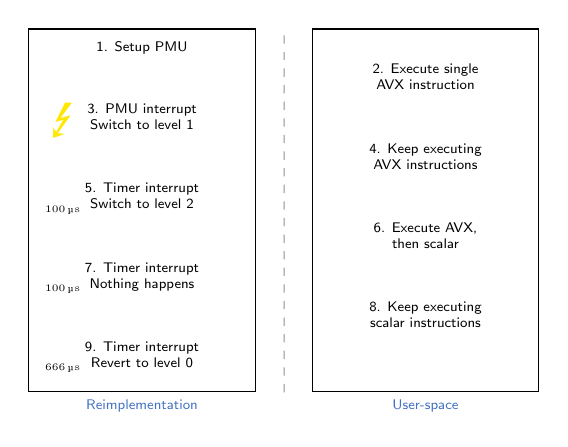
\begin{tikzpicture}[font=\scriptsize,scale=0.72, every node/.style={transform shape}]
	\sffamily
	\pgfmathsetmacro{\componentrectwidth}{4}
	\pgfmathsetmacro{\componentrectheight}{6.4}
	\pgfmathsetmacro{\separatordist}{0.5}
	\pgfmathsetmacro{\arrowoverlength}{0.25}
	\pgfmathsetmacro{\arrowlength}{2*(\arrowoverlength + \separatordist)}
	\pgfmathsetmacro{\halfcomponentrectwidth}{\componentrectwidth*0.5}
	\pgfmathsetmacro{\quartercomponentrectwidth}{\componentrectwidth*0.25}
	
	% kernel
	\draw (0cm,0cm) rectangle ++(\componentrectwidth cm,\componentrectheight) [ref=kernel-rect];
	\node[color=kitblue] at ([yshift=-0.25 cm] kernel-rect south) {Reimplementation};
	
	% separator
	\draw[dashed, color=kitdarkgrey] ([xshift=\separatordist cm] kernel-rect south east) -- ([xshift=\separatordist cm] kernel-rect north east) [ref=separator];
	
	% user-space
	\draw ([xshift=2*\separatordist cm + \componentrectwidth cm] 0, 0) rectangle ++(\componentrectwidth,\componentrectheight) [ref=user-rect];
	\node[color=kitblue] at ([yshift=-0.25 cm] user-rect south) {User-space};
	
	% steps
	\node[align=center, anchor=north] at ([yshift=-0.1cm] kernel-rect north) {1. Setup PMU};
	
	\node[align=center, anchor=north] at ([yshift=-0.5cm] user-rect north) {2. Execute single \\ AVX instruction};
	
	\node[align=center, anchor=north, color=kityellow] at ([yshift=-1.2cm, xshift=-1.4cm] kernel-rect north) {\Huge\Lightning};
	\node[align=center, anchor=north] at ([yshift=-1.2cm] kernel-rect north) {3. PMU interrupt \\ Switch to level 1};
	
	\node[align=center, anchor=north] at ([yshift=-1.9cm] user-rect north) {4. Keep executing \\ AVX instructions};
	
	\node[align=center, anchor=north, color=kitdarkgrey] at ([yshift=-2.55cm, xshift=-1.4cm] kernel-rect north) {\small\Interval};
	\node[align=center, anchor=north] at ([yshift=-3cm, xshift=-1.4cm] kernel-rect north) {\tiny\SI{100}{\micro\second}};
	\node[align=center, anchor=north] at ([yshift=-2.6cm] kernel-rect north) {5. Timer interrupt \\ Switch to level 2};
	
	\node[align=center, anchor=north] at ([yshift=-3.3cm] user-rect north) {6. Execute AVX, \\ then scalar};
	
	\node[align=center, anchor=north, color=kitdarkgrey] at ([yshift=-3.95cm, xshift=-1.4cm] kernel-rect north) {\small\Interval};
	\node[align=center, anchor=north] at ([yshift=-4.4cm, xshift=-1.4cm] kernel-rect north) {\tiny\SI{100}{\micro\second}};
	\node[align=center, anchor=north] at ([yshift=-4cm] kernel-rect north) {7. Timer interrupt \\ Nothing happens};
	
	\node[align=center, anchor=north] at ([yshift=-4.7cm] user-rect north) {8. Keep executing \\ scalar instructions};
	
	\node[align=center, anchor=north, color=kitdarkgrey] at ([yshift=-5.35cm, xshift=-1.4cm] kernel-rect north) {\small\Interval};
	\node[align=center, anchor=north] at ([yshift=-5.8cm, xshift=-1.4cm] kernel-rect north) {\tiny\SI{666}{\micro\second}};
	\node[align=center, anchor=north] at ([yshift=-5.4cm] kernel-rect north) {9. Timer interrupt \\ Revert to level 0};
	\end{tikzpicture}
\end{figure}
\end{frame}

\begin{frame}[t]{Oracle Mechanism}
	\begin{itemize}
		\item Want to find theoretical limit for optimized algorithms
		\begin{itemize}
			\item[$\Rightarrow$] implement oracle mechanism
		\end{itemize}
		\item System call API to tell reimplementation when to switch frequency levels
		\item Synthetic workload with scalar and vector phases
		\begin{itemize}
			\item[$\Rightarrow$] scalar phases of about \SI[quotient-mode=fraction]{2/3}{\milli\second} expose worst case
			\begin{itemize}
				\item hardware's worst case is best case for oracle
			\end{itemize}
			\item Count iterations in each phase
		\end{itemize}
	\end{itemize}
\end{frame}
\section{Evaluation}
\begin{frame}[t]{Reimplementation}
	\begin{itemize}
		\item Need to evaluate correctness and quality of reimplementation
		\begin{itemize}
			\item[$\Rightarrow$] use analysis framework, compare with hardware results
		\end{itemize}
		\item Analysis framework and reimplementation both use performance monitoring
		\begin{itemize}
			\item[$\Rightarrow$] modify analysis kernel module and reimplementation to work together
		\end{itemize}
		\item Measure performance overhead
	\end{itemize}
\end{frame}

\begin{frame}[t]{Model Accuracy}
	\begin{itemize}
		\item Downclocking to level 1 works as expected
		\item Reaching level 2 takes $\approx$ \SI{104}{\micro\second}
		\begin{itemize}
			\item unlike the hardware, we can measure throughput only over time
		\end{itemize}
		\item Upclocking after \SI{666}{\micro\second} as designed
		\begin{itemize}
			\item however, up to \SI{100}{\micro\second} more possible due to limited measurement accuracy
		\end{itemize}
	\end{itemize}
\end{frame}

\begin{frame}[t]{Overhead and Oracle Performance \\ \small AVX phase (\SI[detect-weight=true, detect-family=true]{200}{\milli\second})}
	\begin{figure}
		\centering
		\begin{tikzpicture}[trim axis left, font=\footnotesize]
		\sffamily
		\begin{axis}[
		xlabel={Runs ($n=1000$)},
		ylabel={AVX-512 FMA Loop Iterations},
		scale only axis,
		width=9cm,
		height=3cm,
		axis lines=left,
		ymin=35050000,
		ymax=36200000,
		xtick=\empty,
		xmin=-10,
		xmax=1010,
		legend cell align=left,
		legend style={at={(9cm-9cm/1020*10,0.25)}, anchor=east},
		axis y discontinuity=parallel
		]
		\addplot[only marks, color=kitblue, mark options={scale=0.5}] table {../thesis/plots/staged_execution_0_0_2000000_200000_0_666_avx_hwp.csv}; %node[pos=1.0,below=0.5cm,anchor=east] {Hardware reclocking};
		\addplot[only marks, color=kitgreen, mark options={scale=0.5}] table {../thesis/plots/staged_execution_0_0_2000000_200000_0_666_avx_manual.csv}; %node[pos=1.0,above=0.72cm,anchor=east] {User-space-driven};
		\addplot[only marks, color=kityellow, mark options={scale=0.5}] table {../thesis/plots/staged_execution_0_0_2000000_200000_0_666_avx_avxfreq.csv}; %node[pos=1.0,above=0.67cm,anchor=east] {\textsc{avxfreq}};
		\legend{Hardware,Oracle,Reimplementation}
		\end{axis}
		\end{tikzpicture}
	\end{figure}
	\begin{itemize}
		\item Reimplementation is $\approx$ \SI{1}{\percent} slower in AVX phases
		\item Oracle yields same performance as hardware
	\end{itemize}
\end{frame}

\begin{frame}[t]{Overhead and Oracle Performance \\ \small Scalar phase (\SI[detect-weight=true, detect-family=true]{666}{\micro\second})}
	\begin{figure}
		\centering
		\begin{tikzpicture}[trim axis left, font=\footnotesize]
		\sffamily
		\begin{axis}[
		xlabel={Runs ($n=1000$)},
		ylabel={Scalar Loop Iterations},
		scale only axis,
		width=9cm,
		height=3cm,
		axis lines=left,
		ymin=230000,
		ymax=530000,
		xtick=\empty,
		xmin=-10,
		xmax=1010,
		legend cell align=left,
		legend style={at={(9cm-9cm/1020*10,0.75)}, anchor=east},
		axis y discontinuity=parallel
		]
		\addplot[only marks, color=kitblue, mark options={scale=0.5}] table {../thesis/plots/staged_execution_0_0_2000000_200000_0_666_scalar2_hwp.csv}; %node[pos=1.0,below=0.5cm,anchor=east] {Hardware reclocking};
		\addplot[only marks, color=kitgreen, mark options={scale=0.5}] table {../thesis/plots/staged_execution_0_0_2000000_200000_0_666_scalar2_manual.csv}; %node[pos=1.0,above=0.72cm,anchor=east] {User-space-driven};
		\addplot[only marks, color=kityellow, mark options={scale=0.5}] table {../thesis/plots/staged_execution_0_0_2000000_200000_0_666_scalar2_avxfreq.csv}; %node[pos=1.0,above=0.67cm,anchor=east] {\textsc{avxfreq}};
		\legend{Hardware,Oracle,Reimplementation}
		\end{axis}
		\end{tikzpicture}
	\end{figure}
	\begin{itemize}
		\item Reimplementation $\approx$ \SI{2}{\percent} slower
		\item Oracle gives $\approx$ \SI{8}{\percent} median performance increase (99th percentile: \SI{15}{\percent})
	\end{itemize}
\end{frame}
\section{Future Work}
\begin{frame}[t]{Future Work}
	\begin{itemize}
		\item Implement alternative reclocking algorithms
		\begin{itemize}
			\item Take ideas from power management
		\end{itemize}
		\item More analysis
		\begin{itemize}
			\item Other processors (Haswell, Icelake)
			\item SMT
			\item Instruction mixtures
		\end{itemize}
		\item Reverse engineer AVX frequency offset configuration
	\end{itemize}
\end{frame}
\chapter{Conclusion}
\label{sec:conclusion}

Contemporary Intel processors need to reduce their frequency when executing \gls{AVX} code in order to maintain stability. This has the effect that the performance of heterogeneous workloads with only some specific vectorizable code paths can suffer from these frequency reductions when using \gls{AVX} on these chips. In this work, we wanted to explore the possibility of optimizing Intel's frequency scaling behavior by designing a software-based reimplementation that is supposed to allow us to test alternate algorithms without needing to modify the hardware itself. To be able to do this, we first needed to perform an analysis of the reclocking implementation found in the hardware as there is only very little documentation by Intel available.

In said analysis we found that, for most demanding \gls{AVX} instructions, downclocking is triggered as soon as a single operation was executed and takes about 25 -- \SI{50}{\micro\second}, depending on the heaviness of the executed instructions. As soon as the last instruction has retired, a processor will wait for around \SI[quotient-mode=fraction]{2/3}{\milli\second} before reverting an \gls{AVX}-induced frequency reduction. We used a simplified model based on these results to construct our reimplementation \textsc{avxfreq}, which proved to reflect the model reasonably well. We also were able to show that exploiting an application's knowledge about what it is going to do next can improve performance in a heterogeneous program by \SI{15}{\percent} during scalar phases. However, we also experienced several drawbacks with our reimplementation approach. These include unpredictable delays when raising the frequency, the lack of ways to fully disable the reclocking done by the hardware itself and the impossibility to precisely measure time starting from the point when the last \gls{AVX} instruction in a consecutive streak was executed. Some of these issues may be alleviated or circumvented with further work. As of now, we can not provide a conclusive answer to the feasibility of our idea, as more exploration would be required through implementations of alternative reclocking governors.

\section{Future Work}
\label{sec:conclusion:futurework}

Although we were able to show that improved performance in heterogeneous workloads through better reclocking is theoretically possible, research on this topic is nowhere complete. In this section, we will present several ideas and open issues that may pose interesting topics for future work.

\subsubsection{Alternative reclocking algorithms}
\label{sec:conclusion:futurework:algorithms}

We designed our reimplementation \textsc{avxfreq} with the goal of being able to test alternative reclocking algorithms. So far we implemented a simple design which uses oracle-style foresight to switch frequencies by having user-space programs tell the kernel whenever a phase with \gls{AVX-512} heavy instructions starts or ends. This approach allowed us to estimate what performance improvement may be possible in theoretical best case. However, of course this is not feasible for real-world application as one of the main tasks of an operating system is to hide hardware implementation details such as the need for reclocking from software. We have outlined an approach where the operating system may profile durations of different execution phases in user-space threads to make predictions about the future length of \gls{AVX} and scalar phases that may be used to estimate whether immediately raising the processor's frequency after an \gls{AVX} phase would have a positive impact on overall performance.

\subsubsection{Analysis on other processors}
\label{sec:conclusion:futurework:otherprocessors}

Our analysis in \Cref{sec:analysis} was conducted using an Intel Core i9-7940X processor from the \textit{Skylake (Server)} generation. However, even though older chips from the \textit{Haswell} and \textit{Broadwell} generations only supported \gls{AVX2} and no \gls{AVX-512} \cite{intelhaswell} \cite{intelxeonscalabledeepdive}, they still reduced their frequency when executing demanding \gls{AVX2} instructions, albeit to a smaller extent. Given that we found several discrepancies in the reclocking behavior between what Intel claims in their manuals and what we saw in our analysis results, it may be plausible that Intel's implementation has changed between \textit{Haswell} and \textit{Skylake} and their documentation is simply outdated. Running our tests with a \textit{Haswell} processor could therefore yield interesting insights on why Intel has chosen to implement reclocking the way they did in \textit{Skylake}.

Further, not all \textit{Skylake (Server)} cores are equally equipped with the same amount of \gls{AVX-512} execution units. Our processor had two units per core, whereas other processors from this generation only have one \cite{intelxeonscalabledeepdive}. As more units incur larger power consumption and higher energy density, it is possible that chips which only have one unit per core may behave differently. For the sake of completeness in our analysis and because of potentially different requirements to alternative reclocking algorithms, we should run our framework again on such a processor.

Finally, towards the end of 2019, \textit{Icelake} processors will be the first in the consumer desktop and mobile markets to have \gls{AVX-512} \cite{thicelake}. As Intel makes this instruction set available to a broader range of customers and given that \textit{Icelake} will be the first large microarchitectural overhaul since \textit{Skylake} along with a leap in process technology, they possibly have made changes to their reclocking algorithm. Again, it may be interesting to test our analysis framework on an \textit{Icelake} chip to find potential differences that may have an impact on our and other approaches to optimizing the performance of heterogeneous workloads.

\subsubsection{SMT support in our analysis framework}
\label{sec:conclusion:futurework:smt}

% TODO better reference
As described in \Cref{sec:analysis}, our analysis framework does not support running on processors with \glsreset{SMT}\gls{SMT} enabled. Although we can not conceive of a reason why a processor should behave differently with respect to reclocking when \gls{SMT} is enabled, it is still possible that deviations exist. Given that in nearly all real-world scenarios \gls{SMT} would be enabled, we should implement \gls{SMT} support and verify that there are indeed no differences.

\subsubsection{Huge pages in the analysis user-space component}
\label{sec:conclusion:futurework:hugepages}

In \Cref{sec:analysis:design:userspace} we described how cache coherency effects impacted the results of our analysis framework when run on multiple cores with many pages, each \SI{4}{\kibi\byte} in size. We alleviated the impact by using less pages and instead having a jump at the end to make them loop. However, this theoretically introduces small inaccuracies to the results as the instruction stream becomes slightly heterogeneous. Modern x86 processors alternatively also support pages that are \SI{2}{\mebi\byte} large \cite{intelsdmsysprogguide}, which may be a viable alternative to improve the accuracy of our results.

\subsubsection{Instruction mixtures}
\label{sec:conclusion:futurework:mixtures}

For our analysis, we ran each test using just one specific instruction, repeated many times. However, as Intel hints in their optimization manual \cite{inteloptimizationmanual}, the reclocking is actually triggered depending on the instruction mix executed over a window of several clock cycles. Using data science and machine learning techniques, it may be possible to create a model that can very precisely predict what mixtures will cause a frequency reduction.

\subsubsection{Compiler optimizations using analysis results}
\label{sec:conclusion:futurework:compiler}

Due to the dangers of possible performance degradation for heterogeneous workloads, most compilers do not generate \gls{AVX-512} code unless explicitly instructed to do so \cite{lemire2018avx512}. Even Intel's own C and C++ compiler that previously used to generate \gls{AVX-512} instructions aggressively whenever possible has become very conservative in this regard. With a deeper understanding about when and under what circumstances \gls{AVX}-induced reclocking happens, it may be possible for compilers to make use of \gls{AVX} more often without needing to worry about negative impacts. Thanks to the analysis we have done, much of the required knowledge is now available, while the rest may be achieved through further work as outlined in this chapter.

\subsubsection{Reverse engineering of AVX frequency offsets}
\label{sec:conclusion:futurework:reversing}

In our discussion in \Cref{sec:evaluation:discussion} we have identified the impossibility to completely disable \gls{AVX} reclocking in hardware as a major drawback for our reimplementation approach. However, it is unknown how our motherboard's \gls{UEFI} configures \gls{AVX} frequency offsets in the processor. It may be possible to find out through some reverse engineering efforts though, and this could theoretically reveal a way to achieve full suppression of the processor's own reclocking mechanism.

\subsubsection{Hardware limitations}
\label{sec:conclusion:futurework:hardware}

On Intel \textit{Skylake} \glspl{CPU} it is possible to measure executed floating-point vector instructions, however, no similar performance events exist for other vector instructions. Although this is not within our scope of control, we would like to see event types for all possible types of vector instructions in future processors. It might even make sense to have events that count executed instructions per instruction set. Being able to count all instruction types would be necessary for building a complete reimplementation that can be tested with real-world programs.

Another obstacle preventing a precise software reimplementation of Intel's reclocking algorithm is that we are not able to start measuring time immediately after the last \gls{AVX} instruction has retired. As outlined in \Cref{sec:evaluation:discussion}, a vast improvement here is likely possible with future \textit{Icelake} processors by using improved capabilities of the \gls{PEBS} facility. However, for our purposes it would be optimal if the \gls{PMU} would simply record the \gls{TSC} time-stamp on every assertion of a performance event.

Further, although this is not too much of a problem for us, we are unable to control the power gating of vector registers and vector execution units. In \Cref{sec:evaluation:discussion} we have discussed that the worst conceivable impact are slightly reduced frequencies due to exceeded power budgets. However, it may be interesting to measure the implications of alternative reclocking algorithms for power consumption, which is only inaccurately possible without being able to disable power supply to the gated units upon reverting a frequency reduction.

\end{document}